% =====================================================================
%  Geometry of Forgetting
%  Forgetting as interference: a functional, an optimal-merge identity,
%  and an interference-gated allocation family for continual learning.
%
%  Compile (TeXworks): pdfLaTeX, run twice. Bibliography embedded.
%  Figures: PNG/PDF assets in ./figures.
%  Code & data: https://github.com/j-stoerk/geometry-of-forgetting
% =====================================================================
\documentclass[10pt,a4paper]{article}

\usepackage[utf8]{inputenc}
\usepackage[T1]{fontenc}
\usepackage{lmodern}
\input{glyphtounicode}
\pdfgentounicode=1
\usepackage[margin=2.4cm]{geometry}
\usepackage{graphicx}
\usepackage{amsmath,amssymb}
\usepackage{booktabs}
\usepackage{caption}
\usepackage{enumitem}
\usepackage{xcolor}
\usepackage[hidelinks]{hyperref}
\usepackage{microtype}
\usepackage{amsthm}

\theoremstyle{plain}
\newtheorem{theorem}{Theorem}
\newtheorem{proposition}{Proposition}
\newtheorem{corollary}{Corollary}
\theoremstyle{definition}
\newtheorem{assumption}{Assumption}

\graphicspath{{figures/}}
\captionsetup{font=small,labelfont=bf}
\setlist{itemsep=1pt,topsep=2pt}
\renewcommand{\topfraction}{0.92}
\renewcommand{\bottomfraction}{0.85}
\renewcommand{\textfraction}{0.07}
\renewcommand{\floatpagefraction}{0.75}
\setlength{\textfloatsep}{10pt plus 2pt minus 2pt}

\newcommand{\Sig}{\Sigma}
\newcommand{\Del}{\Delta}
\newcommand{\R}{\mathbb{R}}
\DeclareMathOperator{\range}{range}
\DeclareMathOperator{\Trace}{Tr}
\newcommand{\sstar}{s^{\ast}}
\newcommand{\IGFA}{igfa}
\newcommand{\OGD}{\textsc{ogd}}

\title{\textbf{Forgetting as Interference in Continual Learning:
Optimal Merging and Interference-Gated Allocation}}

\author{Julius St\"ork$^{1,2,\ast}$\\[2pt]
\small $^1$VARTA Microbattery GmbH, Ellwangen, Germany\\
\small $^2$Technische Universit\"at Braunschweig, Braunschweig, Germany\\
\small $^\ast$Corresponding author: \texttt{julius.stoerk@varta-ag.com}\\[2pt]
\small \textit{Draft manuscript, \today}}
\date{}

\begin{document}
\maketitle

% =====================================================================
\begin{abstract}
\noindent
Continual learning commonly relies on post-hoc mechanisms such as replay, elastic
regularization, or distillation, which mitigate interference only after it has
occurred. This work instead models interference directly. In frozen-feature,
linear heads, forgetting equals interference energy $\tfrac12\,\Del^\top\Sig_A\Del$ induced by a later update
$\Del$, measured in the earlier task's input covariance $\Sig_A$. This identity extends to deep networks by measuring curvature along the path of the task loss, with only a small number of additional forward passes.

Two consequences follow. First, interference is removable when task supports are
disjoint ($\Del\in\ker\Sig_A$); otherwise a non-zero distortion floor is
unavoidable and is given by the posterior-variance-weighted target gap, with
corresponding mutual-information bounds. Second, optimal model merging reduces to
$\Sig$-orthogonalization of task vectors, and continual learning can be interpreted
as its online greedy analogue.

Based on this view, this work introduces Interference-Gated Functional
Allocation (\IGFA), a replay-free, Fisher-free method that shares
capacity when a regime-specific task similarity exceeds $\sstar\approx0.26$ and orthogonalizes updates under conflict.
Empirically, \IGFA{} yields lossless retention on disjoint supports and shifts
unavoidable forgetting into deferred but recoverable plasticity. On Split-Digits it
matches or exceeds strong replay-free and Fisher-free baselines, achieving $0.98$
accuracy with near-zero forgetting using only a low-rank state summary. On
Split-CIFAR-100 with a frozen ViT it reaches parity with the strongest structural
baseline at the best retention level, without replay or Fisher information; on ImageNet-R
its signed gate significantly exceeds unconditional projection at equal forgetting. At
billion-parameter scale with \texttt{pythia-1b}, continual pretraining shows the
same replay-free, Fisher-free retention mechanism achieving the lowest loss and the
least forgetting, while a pre-flight diagnostic correctly predicts when retention is
feasible.
\end{abstract}

\vspace{1ex}
\noindent\textbf{Keywords:} continual learning; catastrophic forgetting; model
merging; neural tangent kernel; gradient projection; rate--distortion; representation geometry

\begin{figure}[t]\centering
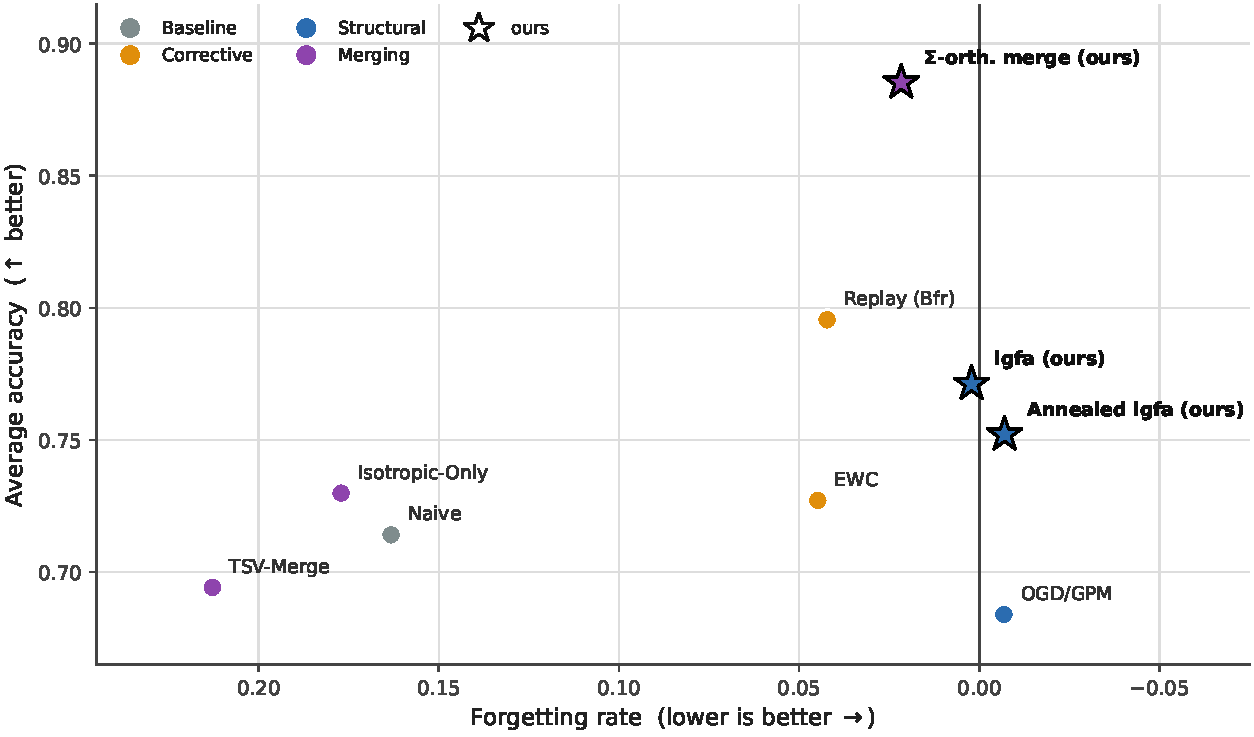
\includegraphics[width=0.9\textwidth]{fig_teaser}
\caption{\textbf{Accuracy versus forgetting.}  Nine methods on
the exact-A1 Rotated-Digits benchmark (five rotations, frozen random features; mean over
$5$ seeds) are differentiated by method class (baseline / corrective / structural / merging); our
methods are marked ``(ours)''; higher accuracy (up) and lower forgetting (right) are better. \emph{Corrective}
(EWC, replay) and \emph{online structural} (\OGD{}/\textsc{gpm}, \IGFA) methods learn the
stream sequentially, whereas \emph{merging} methods solve each rotation independently and
combine offline. 
\emph{(i)} The $\Sig$-orthogonal merge of Theorem~\ref{thm:merge} attains near-oracle accuracy
($0.885$ against a $0.903$ per-task ceiling) with the smallest
post-merge residual floor ($D=0.032$, versus $0.20$ and $0.38$ for the isotropic and
Euclidean merges), confirming that the task-induced, non-Euclidean $\Sig$-metric
is the correct inner product for merging. \emph{(ii)} Among online, buffer- and
Fisher-free methods, our signed gate (\IGFA) attains the highest accuracy; annealing the
protection boundary (Annealed \IGFA) trades slightly lower accuracy for lower, even negative,
forgetting. Full numbers
with confidence intervals and the residual-$D$ ablation are in Sec.~\ref{si:compare}.}
\label{fig:teaser}
\end{figure}

% =====================================================================
\section{Introduction}
\label{sec:intro}

A model trained sequentially on task $B$ after task $A$ often degrades on task $A$,
a phenomenon known as catastrophic forgetting. Networks trained by stochastic gradient
descent (SGD) or its variants update from the current minibatch alone (or a smoothed
average of a short window of minibatches); the update is therefore \emph{oblivious to past
knowledge}. This obliviousness is desirable when the training data are
i.i.d., but harmful once the training distribution shifts over time in the continual
setting. Standard approaches such as replay
\cite{lopezpaz2017,chaudhry2019,buzzega2020}, elastic weight consolidation
\cite{kirkpatrick2017,zenke2017}, and distillation \cite{li2017lwf} mitigate this
effect after interference has occurred. Although effective, these methods are
primarily corrective: replay requires data storage and may raise privacy concerns,
regularization constrains plasticity, and none directly characterizes when
interference is unavoidable and when it can be eliminated.

The analysis focuses on the regime in which
a frozen feature extractor $\phi(x)$ is paired with a trainable linear head,
covering the common frozen-backbone and parameter-efficient fine-tuning
(PEFT) settings and the first-order neural tangent \cite{jacot2018} approximation of
a fully trained network.
The forgetting of an earlier task $A$ after an
update $\Del$ caused by learning task $B$
is exactly the interference energy
$\tfrac12\,\Del^\top\Sig_A\Del$, where $\Sig_A\ = \mathbb{E}_{x \sim D_A}\left[\phi(x)\phi(x)^\top\right]$ denotes the feature second moment of task
$A$, measuring which feature directions are active for that task.
The same geometry predicts per-task forgetting accurately and
extends approximately to deeper networks with feature drift.

The functional has three consequences. First, the
geometry of $\Sig_A$ only penalizes components in its active subspace and
does not change task $A$'s loss for updates in the null space
$\ker\Sig_A$. Interference is removable for disjoint task supports (reduces to ordinary orthogonality in isotropic geometry),
whereas overlapping supports imply a non-zero distortion floor.
Second, the same functional gives an optimality condition for model merging: task
vectors should be orthogonal under the $\Sig$-induced metric, which makes offline
merging and online continual learning two scheduling variants of the same objective.
Third, it motivates Interference-Gated Functional Allocation (\IGFA), an online
method that uses a low-rank summary of the occupied function subspace to decide
whether a new update should be shared or orthogonalized
(Fig.~\ref{fig:overview}).

\begin{figure}[tb]\centering
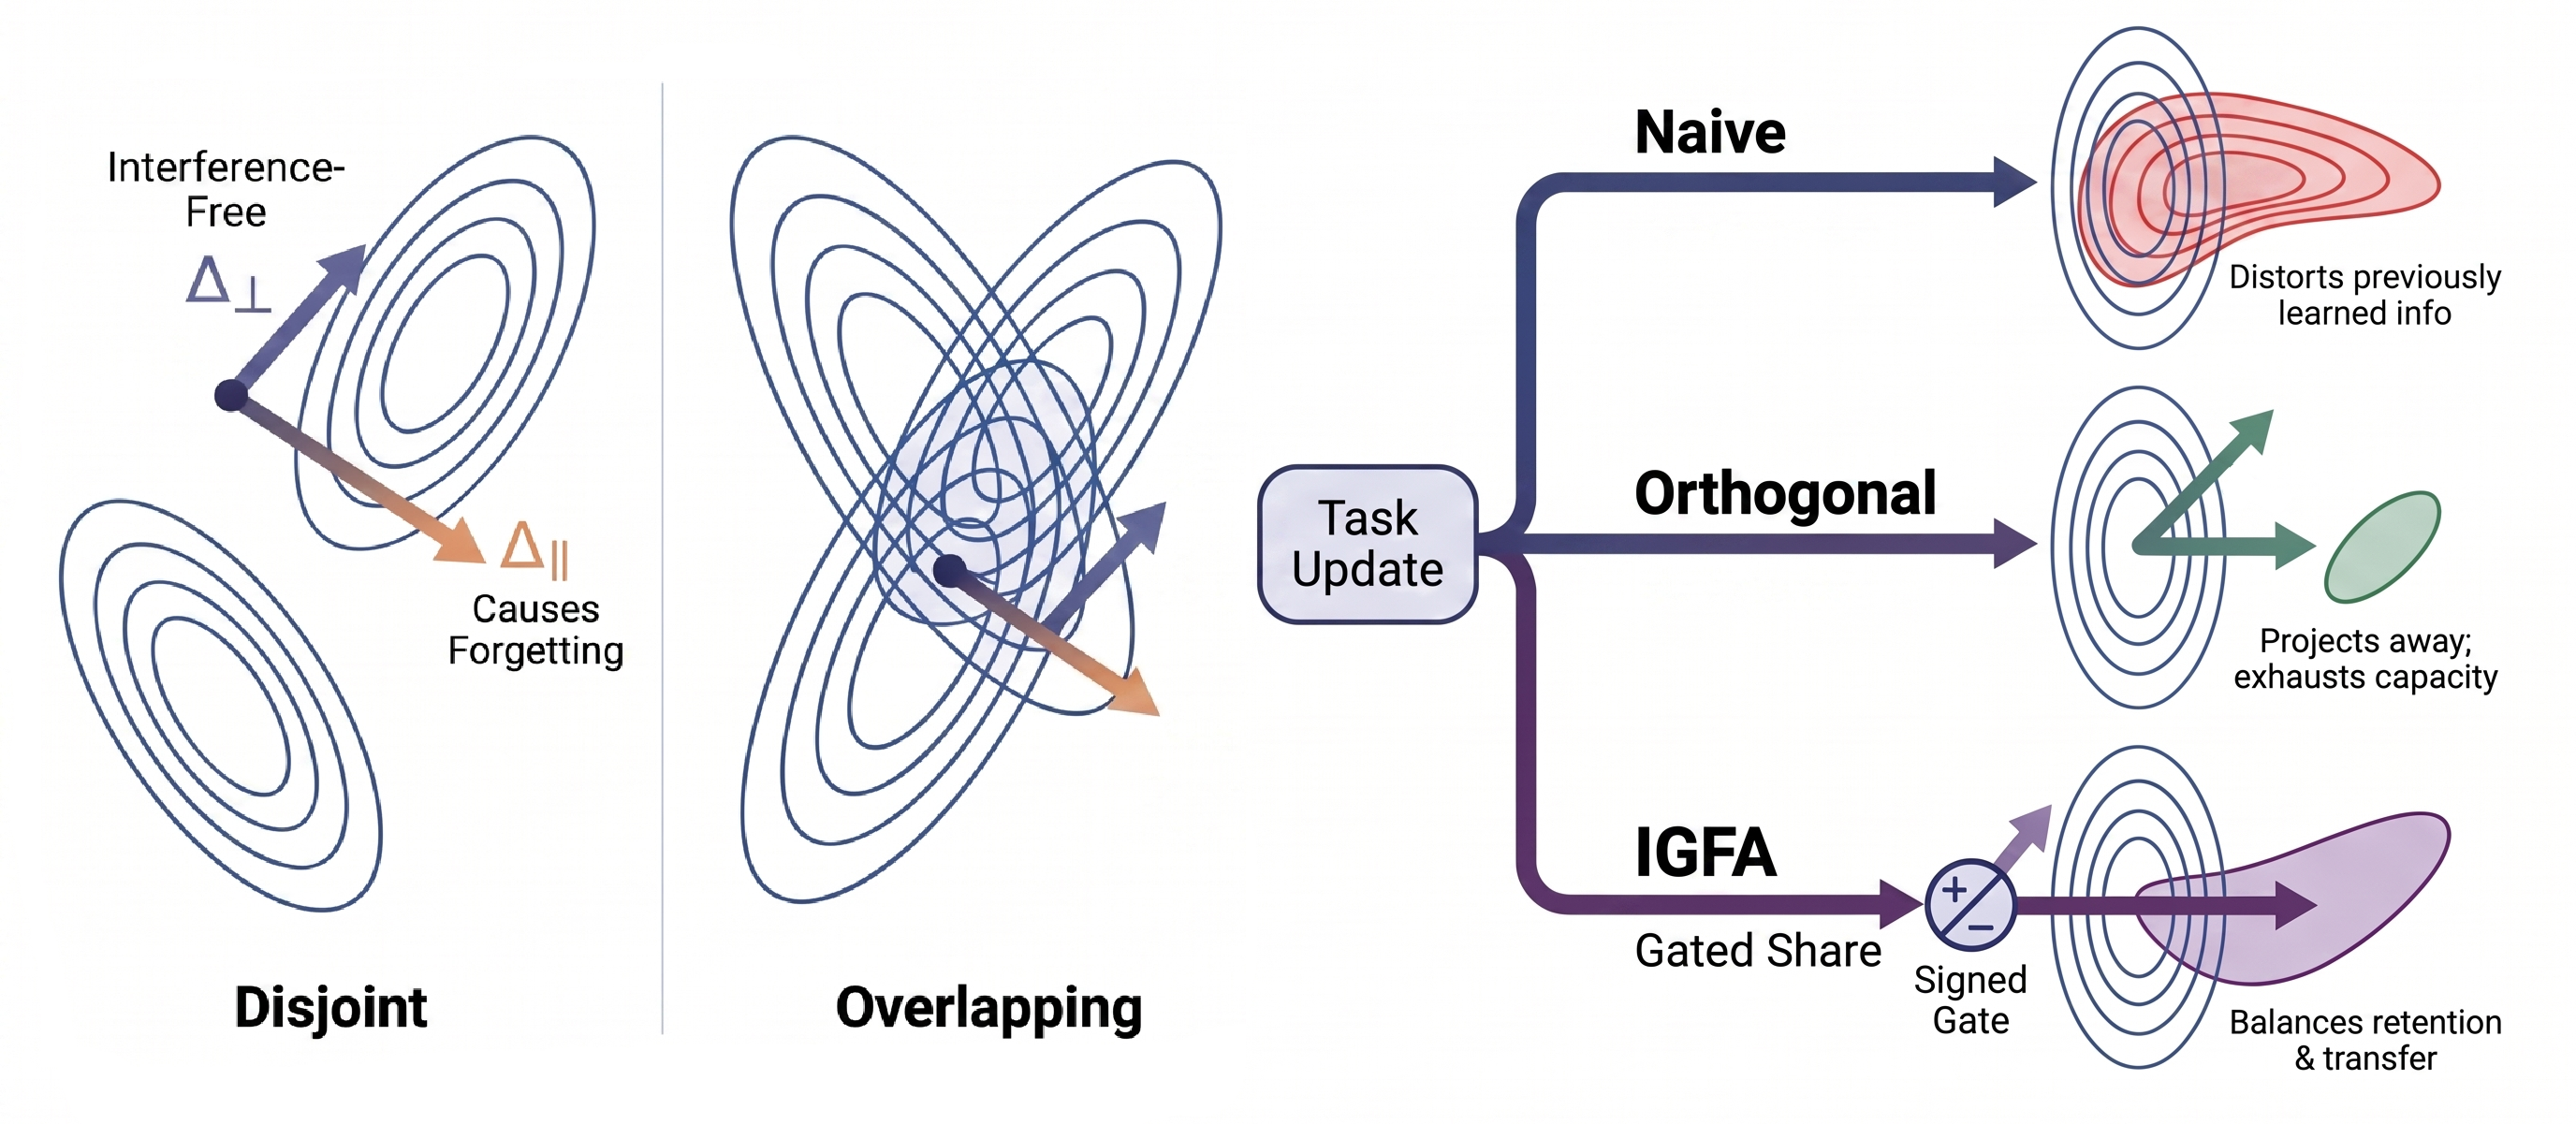
\includegraphics[width=\textwidth]{Subspace_Interference_and_Forgetting_Geometry}
\caption{The task-induced geometry in feature space motivates either full sharing, full separation, or selective parameter sharing.
\emph{Left (Disjoint).} When two tasks excite orthogonal feature subspaces, the
update $\Del=\Del_\parallel+\Del_\perp$ splits into a component
$\Del_\parallel\in\range\Sig_A$ across the iso-loss contours (the only part that
costs forgetting) and $\Del_\perp\in\ker\Sig_A$ (interference-free); allocation is
lossless. \emph{Centre (Overlapping).} When the supports share an active direction,
no update for $B$ can avoid $\range\Sig_A$ and a distortion floor is unavoidable.
\emph{Right.} The same functional yields three update rules. Naive descent
incurs the full interference (distorts old knowledge); orthogonal
projection (\OGD{}/\textsc{gpm} \cite{farajtabar2020,saha2021}) removes all overlap
(no forgetting, but no transfer and capacity exhaustion); \IGFA{} applies a
\emph{signed} gate---sharing aligned directions and orthogonalizing conflicting
ones---balancing retention and transfer while carrying only the occupied subspace as
state.}
\label{fig:overview}
\end{figure}

The paper makes three contributions.
\begin{enumerate}[leftmargin=1.6em,itemsep=3pt]
\item \textbf{Interference functional and removability.} Section~\ref{sec:theory}
shows that forgetting is exactly the interference energy induced by a later update.
This yields a structural criterion for lossless retention and identifies the
unavoidable distortion floor when task supports overlap. The same quantity admits an
information-theoretic interpretation through the task-inference problem.
\item \textbf{Optimal merging as $\Sig$-orthogonalization.}
Section~\ref{sec:theory:merge} shows that post-merge loss decomposes into task-wise
fit and cross-task interference. Minimizing this objective requires mutual
$\Sig$-orthogonality of the task vectors, linking model merging and continual
allocation under a common geometric principle.
\item \textbf{Interference-Gated Functional Allocation.} Section~\ref{sec:algo}
introduces \IGFA, a replay-free and Fisher-free online algorithm that stores only a
low-rank subspace summary. Unlike unconditional orthogonal projection methods,
\IGFA{} shares capacity when tasks are sufficiently aligned and orthogonalizes
updates only when interference is predicted.
\end{enumerate}

All formal results are established in the linear-on-features regime. The experiments
in Section~\ref{sec:exp} are designed to test the theory directly, including lossless
allocation on disjoint supports, the relocation of unavoidable cost from forgetting
into deferred plasticity, the similarity threshold at $\sstar\approx0.26$, and the
onset of a capacity floor once the cumulative occupied rank reaches the feature
dimension, $T\,r\approx d$ (with $T$ the number of tasks in the stream, $r$ the
rank of the feature subspace each task occupies, and $d$ the feature dimension).
In the frozen-feature Split-Digits
setting, \IGFA{} matches the strongest replay-free and Fisher-free baseline at about
$0.98$ accuracy with near-zero forgetting while using no replay buffer.
Extensions to
full-network training, large-scale overlays, and direct comparison with replay at
scale are discussed in Section~\ref{sec:discussion}, with the supporting experiments
detailed in the Supporting Information.

% =====================================================================
\section{Related work}
\label{sec:related}

\paragraph{Corrective continual learning.} Replay, regularization, and distillation
remain the main corrective approaches to continual learning
\cite{lopezpaz2017,chaudhry2019,buzzega2020,kirkpatrick2017,zenke2017,li2017lwf}.
They are effective baselines, but they do not explicitly model interference through
task geometry. In contrast, the interference functional derived below predicts the
collision and identifies when it can be removed before it occurs; replay can be
viewed as a stochastic Monte-Carlo estimator of the same task second-moment $\Sig_t$
that we summarize directly via a low-rank subspace.

\paragraph{Geometry- and gradient-based methods.} A related line of work controls the
update direction itself. Orthogonal Gradient Descent \cite{farajtabar2020}, Gradient
Projection Memory \cite{saha2021}, and Orthogonal Weight Modification
\cite{zeng2019owm} project updates away from subspaces associated with previous
tasks; in the present setting this corresponds to enforcing $\Del\in\ker\Sig_A$.
PCGrad-style methods \cite{yu2020pcgrad} resolve conflicts through pairwise gradient
comparisons rather than explicit task-subspace protection. Recent work also studies
closely related regimes: Geodesic-Aligned Gradient Projection \cite{geodesic2025}
addresses feature drift during sequential learning, and MINGLE \cite{mingle2025} uses
a null-space criterion to gate low-rank experts during test-time merging. Relative to
these approaches, the present framework derives the projection condition from an exact
forgetting functional, replaces unconditional projection with a similarity-based
share-or-orthogonalize rule, and uses the same functional to characterize both
merging and the distortion floor. NTK-based analyses \cite{doan2021,bennani2020}
likewise relate forgetting to overlap in representation space, but do not develop the
$\Sig$-orthogonality criterion or the associated transfer gate.

\paragraph{Model merging and task arithmetic.} A parallel literature merges
independently fine-tuned models through arithmetic on weight-space task vectors
\cite{ilharco2023,yadav2023}. These methods usually operate in Euclidean parameter
space, whereas the present analysis identifies the task-dependent metric induced by
$\Sig_t$ as the relevant geometry. Under this metric, optimal merging becomes mutual
$\Sig$-orthogonalization, with ordinary weight-space orthogonality recovered only when
$\Sig_t\propto I$. Task Singular Vectors \cite{gargiulo2025tsv} promotes orthogonality
by whitening singular directions of task vectors; by contrast, isotropic merging
\cite{marczak2025iso} shows that shared-subspace isotropy can outperform strict
orthogonalization. WUDI-Merging \cite{cheng2025wudi} is particularly close in spirit
because it links task vectors to input subspaces and minimizes interference without
data; the key difference here is that the metric and residual are \emph{derived} from
an exact forgetting functional rather than an approximate subspace argument.
Tangent-space continual merging \cite{holistic2026} also operates in a first-order
regime, but with similar trade-offs between scalability and functional specificity.
The common perspective adopted here is that the same interference functional governs
both offline merging and online continual allocation.

\paragraph{Scenarios, scale, and plasticity.} The standard task-, domain-, and
class-incremental taxonomy \cite{vandeven2022} distinguishes whether task identity is
given or must be inferred. In this context, the distortion floor developed later
provides a quantitative link between support overlap and task inference. Related
empirical and analytical work has examined the effects of scale and pretraining
\cite{ramasesh2022}, frozen-backbone prompt and adapter methods
\cite{wang2022l2p,wang2022dualprompt,smith2023coda}---which learn prompt pools with
input-conditioned selection under a class-incremental protocol and provide strong empirical
accuracy without structural retention guarantees (differentiated in
Sec.~\ref{sec:exp:cifar})---forgetting in linear models
\cite{evron2022}, plasticity loss \cite{dohare2024}, and convergence or task ordering
in continual linear classification \cite{jung2025,lihiratani2025}.

% =====================================================================
\section{Preliminaries: the interference functional}
\label{sec:theory}
This section fixes the setting and assumptions (Sec.~\ref{sec:theory:setup}), derives the
interference functional and the removability dichotomy (Sec.~\ref{sec:theory:functional}),
generalizes the identity beyond frozen features (Sec.~\ref{sec:theory:general}), and derives
the optimal merge together with the distortion floor (Sec.~\ref{sec:theory:merge}).

\begin{figure}[tb]\centering
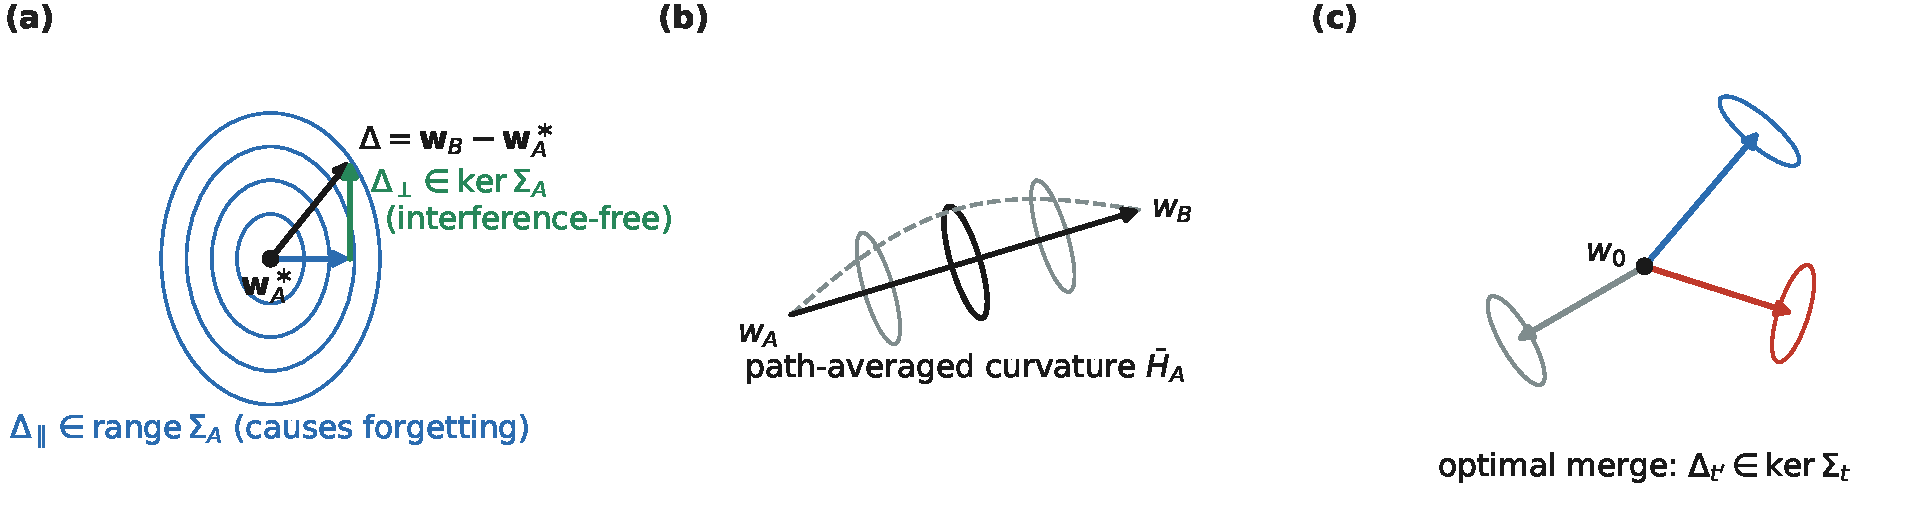
\includegraphics[width=\textwidth]{thm_geometry}
\caption{Geometry of the core identities. \emph{(a)} Forgetting is the interference
energy $\tfrac12\Del^\top\Sig_A\Del$; only the component $\Del_\parallel\in\range
\Sig_A$ costs forgetting, while $\Del_\perp\in\ker\Sig_A$ is free
(Theorem~\ref{thm:functional}). \emph{(b)} For general architectures the input
covariance is replaced by the path-averaged curvature $\bar H_A$ along the segment
$w_A\!\to\!w_B$ (Theorem~\ref{thm:general}). \emph{(c)} Optimal merging makes the
task vectors mutually $\Sig$-orthogonal (Theorem~\ref{thm:merge}).}
\label{fig:thmgeom}
\end{figure}

\subsection{Setting and assumptions}
\label{sec:theory:setup}
Let $\phi:\mathcal X\to\R^d$ be a fixed feature map and $w\in\R^d$ a trainable linear
head with prediction $\hat y=w^\top\phi(x)$. For task $t$, let
$\Sig_t=\mathbb{E}_{x\sim\mathcal D_t}[\phi(x)\phi(x)^\top]\succeq0$ denote the feature
second moment, and let $w_t^\ast$ be a realizable optimum. The per-task excess loss is
\begin{equation}
L_t(w)=\tfrac12\,(w-w_t^\ast)^\top\Sig_t\,(w-w_t^\ast)\;\ge 0.
\label{eq:excess}
\end{equation}
Equation~\eqref{eq:excess} is exactly the excess population risk under squared loss.
Writing $y=\phi(x)^\top w_t^\ast+\varepsilon$ with $\mathbb{E}[\varepsilon]=0$ and
$\varepsilon\!\perp\!\phi(x)$ gives $\mathbb{E}[(\hat y-y)^2]/2=L_t(w)+\tfrac12
\mathbb{E}[\varepsilon^2]$, so all loss differences below depend only on $L_t(w)$. Three
assumptions fix the regime: \textbf{(A1) frozen features}---$\phi$ is fixed during training,
exact for frozen-backbone and PEFT settings and the first-order NTK \cite{jacot2018} model of
end-to-end training, so full-network claims are first-order and are tested in
Sec.~\ref{sec:exp:breakdown}; \textbf{(A2) realizability}---each $w_t^\ast$ attains zero
excess loss, so mis-specification adds only a task-constant and leaves the interference terms
untouched; and \textbf{(A3) the quadratic regime}---training minimizes Eq.~\eqref{eq:excess}
by (projected) gradient descent, so motion is confined to the excited subspace while
directions in $\ker\Sig_t$ leave $L_t$ unchanged.

\subsection{The functional and the removability dichotomy}
\label{sec:theory:functional}
Train task $A$ from a base point $w_0$ to convergence. Under A3, gradient descent
moves only in $\range\Sig_A$, so the converged solution $w_A$ satisfies $L_A(w_A)=0$
and equals $w_A^\ast$ up to an arbitrary component in $\ker\Sig_A$. For loss
differences we therefore take $w_A=w_A^\ast$. Now train task $B$, reaching $w_B$, and
define $\Del=w_B-w_A^\ast$.

\begin{theorem}[Forgetting is interference energy]
\label{thm:functional}
Under A1--A3, the forgetting of task $A$ caused by learning $B$ is
\begin{equation}
\Del L_A=L_A(w_B)-L_A(w_A^\ast)=\tfrac12\,\Del^\top\Sig_A\,\Del,
\qquad \Del=w_B-w_A^\ast.
\label{eq:functional}
\end{equation}
\end{theorem}
\begin{proof}
Since $L_A(w_A^\ast)=0$ by A2, substituting $w_B=w_A^\ast+\Del$ into
Eq.~\eqref{eq:excess} yields $L_A(w_B)=\tfrac12\Del^\top\Sig_A\Del$. No approximation
is involved; the only essential assumption is that $\phi$ remains fixed, so $\Sig_A$
is unchanged before and after learning $B$.
\end{proof}

\noindent Decompose the update as $\Del=\Del_\parallel+\Del_\perp$, with
$\Del_\perp\in\ker\Sig_A$ and $\Del_\parallel\in\range\Sig_A$. Then $\Del L_A=
\tfrac12\Del_\parallel^\top\Sig_A\Del_\parallel$, so only the component of the update
lying in task $A$'s active subspace contributes to forgetting
(Fig.~\ref{fig:thmgeom}a).

\begin{corollary}[Removability dichotomy]
\label{cor:removability}
An update is lossless for $A$ if and only if $\Del\in\ker\Sig_A$. Consequently there
exists a way to learn $B$ with zero forgetting of $A$ if $w_B^\ast$ is reachable
through $\ker\Sig_A$, i.e. if $w_B^\ast-w_A^\ast\in\ker\Sig_A$. Even when this fails,
$L_B$ can still be strictly reduced without forgetting whenever $w_B^\ast-w_A^\ast$ has
a non-zero component in $\ker\Sig_A\cap\range\Sig_B$. If $\range\Sig_A$ and
$\range\Sig_B$ share an active direction on which $w_A^\ast$ and $w_B^\ast$ disagree,
then no lossless update reaches $w_B^\ast$, and a positive floor remains
(Theorem~\ref{thm:floor}).
\end{corollary}
\begin{proof}
Since $\Sig_A\succeq0$, $\Del^\top\Sig_A\Del=0\Leftrightarrow\Sig_A^{1/2}\Del=0
\Leftrightarrow\Del\in\ker\Sig_A$. Projected gradient descent on $L_B$ restricted to
$w_A^\ast+\ker\Sig_A$ converges to the minimizer on that affine set. It reaches
$w_B^\ast$ if $w_B^\ast-w_A^\ast\in\ker\Sig_A$, and it strictly reduces $L_B$ whenever
the projection of $-\nabla L_B(w_A^\ast)$ onto $\ker\Sig_A$ is non-zero, equivalently
whenever $\Sig_B(w_B^\ast-w_A^\ast)$ has a non-zero component in $\ker\Sig_A$. In the
disjoint-support case, $\range\Sig_B\subseteq\ker\Sig_A$, so the entire update is
lossless.
\end{proof}

Here, ``task support'' refers to the column space $\range\Sig_t$, that is, the
subspace of feature directions activated by task $t$. Disjoint supports therefore mean
orthogonal feature subspaces, not disjoint label sets.

\subsection{The architecture-general identity}
\label{sec:theory:general}
Theorem~\ref{thm:functional} assumes frozen features. In end-to-end training, feature
drift degrades the frozen-curvature prediction, especially in deeper networks and at
larger step sizes. The correct generalization is to replace $\Sig_A$ by the curvature
of $L_A$ averaged along the displacement from $w_A$ to $w_B$.

\begin{theorem}[Architecture-general forgetting identity]
\label{thm:general}
Let $L_A$ be any twice-differentiable task-$A$ loss, and let training on $B$ move the
parameters from $w_A$ to $w_B$. Writing $\Del=w_B-w_A$,
\begin{equation}
\Del L_A=\nabla L_A(w_A)^\top\Del+\tfrac12\,\Del^\top \bar H_A\,\Del,
\qquad
\bar H_A=2\!\int_0^1(1-t)\,\nabla^2 L_A(w_A+t\Del)\,dt,
\label{eq:general}
\end{equation}
where $\bar H_A$ is the Hessian of $L_A$ averaged along the segment $w_A\!\to\!w_B$. If
$w_A$ is a stationary point, then $\nabla L_A(w_A)=0$ and
$\Del L_A=\tfrac12\Del^\top\bar H_A\Del$.
\end{theorem}
\noindent\emph{Intuition:} a second-order Taylor expansion of $L_A$ along the segment
$w_A\!\to\!w_B$, with exact integral remainder, produces the gradient term and the
path-averaged Hessian (full derivation in Sec.~\ref{si:proofs}).

\noindent Theorem~\ref{thm:functional} is the constant-curvature special case: if
$\nabla^2 L_A\equiv\Sig_A$ then $\bar H_A=\Sig_A$. For squared loss,
$\nabla^2 L_A(w)=\mathbb{E}_{\mathcal D_A}[J_w J_w^\top]+R(w)$, so $\bar H_A$ is a
path-averaged Gauss--Newton geometry, where $J_w=\partial f(x;w)/\partial w$ is the
parameter Jacobian and $R(w)$ is a residual-curvature term (Fig.~\ref{fig:thmgeom}b).
The removability, merging, and floor results therefore extend by replacing $\Sig_A$
with $\bar H_A$. In practice, $\bar H_A$ can be estimated from a small number of
evaluations of $L_A$ along the segment, without forming the Hessian explicitly. The
same prescription tells \IGFA{} what to track under drift: the running Gauss--Newton
subspace $\mathbb{E}[J_w J_w^\top]$ rather than a stale $\Sig_A$.

\subsection{Optimal Merging and the Distortion Floor}
\label{sec:theory:merge}
Represent $K$ task solutions as $\Del_t=w_t^\ast-w_0$ from a shared base $w_0$, and
merge them as $\theta^\ast=w_0+\sum_t\Del_t$. Substituting into
Eq.~\eqref{eq:excess}, the loss incurred on task $t$ is
\begin{equation}
L_t(\theta^\ast)=\tfrac12\Big(\textstyle\sum_{t'\neq t}\Del_{t'}\Big)^{\!\top}
\Sig_t\Big(\textstyle\sum_{t'\neq t}\Del_{t'}\Big),
\label{eq:merge-energy}
\end{equation}
that is, the interference energy of the other task vectors measured in task $t$'s
geometry.

\begin{theorem}[Optimal merging is $\Sig$-orthogonalization]
\label{thm:merge}
The total merge loss $\sum_t L_t(\theta^\ast)$ vanishes whenever the task vectors are
pairwise $\Sig$-orthogonal, i.e. $\Del_{t'}\in\ker\Sig_t$ for all $t'\neq t$; this
condition is also generically necessary. When it fails, the minimum total loss over
shared heads is attained at
$\theta_J=\big(\sum_t\Sig_t\big)^{+}\big(\sum_t\Sig_t w_t^\ast\big)$, and for two
tasks
\begin{equation}
w_J=(\Sig_A+\Sig_B)^{+}(\Sig_A w_A^\ast+\Sig_B w_B^\ast).
\label{eq:merge-two}
\end{equation}
The residual $\mathcal{D}:=\sum_t L_t(\theta_J)$ is the \emph{distortion floor}.
\end{theorem}
\begin{proof}
Since each $L_t(\theta^\ast)\ge0$, the sum vanishes iff every term vanishes, i.e.
$\Sig_t^{1/2}\sum_{t'\neq t}\Del_{t'}=0$. A sufficient, and generically necessary,
condition is $\Del_{t'}\in\ker\Sig_t$ for all $t'\neq t$. The minimizer of $\sum_t
L_t(\theta)=\tfrac12\sum_t(\theta-w_t^\ast)^\top\Sig_t(\theta-w_t^\ast)$ satisfies
$\sum_t\Sig_t(\theta-w_t^\ast)=0$, which gives $\theta_J$; Eq.~\eqref{eq:merge-two} is
the two-task case.
\end{proof}

\noindent The relevant inner product for merging is therefore the task-dependent
$\Sig_t$-metric rather than the Euclidean metric of parameter space
(Fig.~\ref{fig:thmgeom}c); Euclidean orthogonality is the white-feature special case
$\Sig_t\propto I$. The same residual $\mathcal{D}$ also governs the online
continual-learning setting, so merging and continual learning optimize the same
functional on different schedules.

\paragraph{When orthogonality fails: the distortion floor.}\label{sec:theory:ceiling}
Optimal merging requires $\Sig$-orthogonality; when the supports force it to fail, the
residual $\mathcal{D}$ of Theorem~\ref{thm:merge} does not vanish, and it has a
task-inference reading. Consider two tasks as a single problem in which each input carries a
hidden label $T\in\{A,B\}$, and a shared head must predict the task-appropriate target.

\begin{figure}[tb]\centering
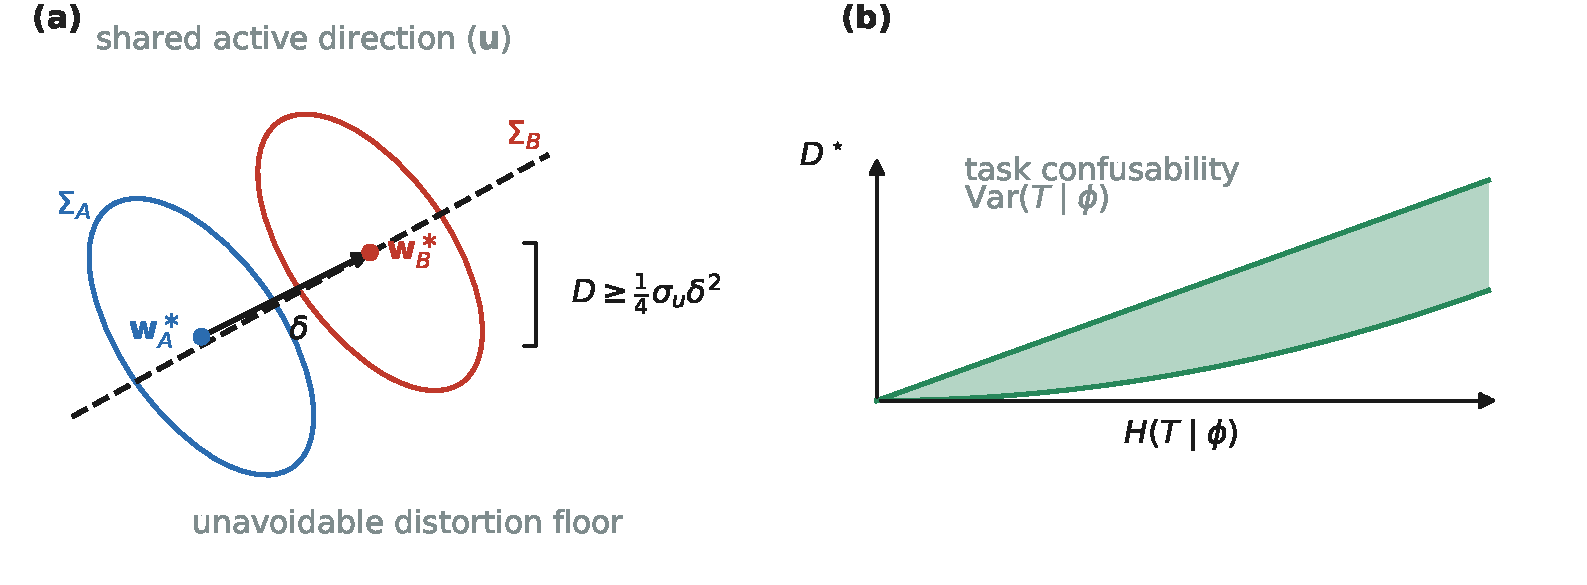
\includegraphics[width=\textwidth]{thm_floor}
\caption{The distortion floor and its information-theoretic reading.
\emph{(a)} A floor appears only on a shared active direction $u\in\range\Sig_A\cap
\range\Sig_B$ on which the targets disagree by $\delta$, with
$\mathcal{D}\ge\tfrac14\sigma_u\delta^2$ (Theorem~\ref{thm:floor}).
\emph{(b)} The Bayes single-head excess risk $\mathcal{D}^\star$ factors into the
geometric target gap $(\phi^\top\delta)^2$---the displacement $\delta$ in (a)---and the
task-confusability factor $\operatorname{Var}(T\!\mid\!\phi)$, which is two-sidedly
controlled by the conditional entropy $H(T\!\mid\!\phi)$ (Theorem~\ref{thm:mi}; band).}
\label{fig:thmfloor}
\end{figure}

\begin{theorem}[Distortion floor and inference obstruction]
\label{thm:floor}
Suppose the tasks share an active direction $u$, with $\|u\|=1$ and
$u\in\range\Sig_A\cap\range\Sig_B$, and let $\delta=u^\top(w_B^\ast-w_A^\ast)$. Then
the distortion floor obeys the lower bound
\begin{equation}
\mathcal{D}\ \ge\ \tfrac14\,\sigma_u\,\delta^2,\qquad
\sigma_u=\big(u^\top(\Sig_A^{-1}+\Sig_B^{-1})u\big)^{-1},
\label{eq:floor-bound}
\end{equation}
where $\Sig_A^{-1}$ and $\Sig_B^{-1}$ denote the inverses of $\Sig_A$ and $\Sig_B$
restricted to the shared active subspace $S=\range\Sig_A\cap\range\Sig_B$. On the
shared support, the excess Bayes risk of the Bayes-optimal single head over the task
oracle equals the merge residual.
\end{theorem}
\noindent\emph{Intuition:} restricting the merge to the shared direction $u$ reduces it to a
scalar two-point problem whose $\Sig$-weighted optimum leaves residual
$\tfrac14\sigma_u\delta^2$; summing over shared directions and identifying the Bayes single
head with the posterior mean gives the bound and the inference claim (Sec.~\ref{si:proofs}).

\noindent Support overlap is therefore the common obstruction to both
$\Sig$-orthogonal merging and task inference; a positive floor appears only on shared
active directions where the tasks also disagree. This yields the geometric counterpart
of the task- versus class-incremental distinction \cite{vandeven2022}: disjoint
supports make the task identity effectively free, whereas overlapping supports can
induce a non-zero floor when the tasks disagree on shared active directions.

\begin{theorem}[Information--estimation identity for the floor]
\label{thm:mi}
Let $T\sim\mathrm{Unif}\{A,B\}$, $\phi\mid T\sim\mathcal D_T$,
$y=\phi^\top w_T^\ast+\varepsilon$, with $\varepsilon\perp(T,\phi)$,
$\mathbb{E}\varepsilon=0$, and $\mathbb{E}\varepsilon^2=\sigma^2$. Writing
$\eta(\phi)=\Pr(T{=}A\mid\phi)$ and $\delta=w_A^\ast-w_B^\ast$, the excess Bayes risk
of a single shared head over the task oracle is
\begin{equation}
\mathcal{D}^\star
=\tfrac12\,\mathbb{E}_\phi\!\big[\operatorname{Var}(T\!\mid\!\phi)\,(\phi^\top\delta)^2\big]
=\tfrac12\,\mathbb{E}_\phi\!\big[\eta(1-\eta)\,(\phi^\top\delta)^2\big].
\label{eq:mi-identity}
\end{equation}
With $h_b(p)=-p\ln p-(1-p)\ln(1-p)$ the binary entropy in nats, this implies the
two-sided bounds
\begin{equation}
\tfrac18\,\mathbb{E}_\phi\!\big[(\phi^\top\delta)^2\,h_b(\eta)^2\big]\ \le\
\mathcal{D}^\star\ \le\
\tfrac14\,\mathbb{E}_\phi\!\big[(\phi^\top\delta)^2\,h_b(\eta)\big].
\label{eq:mi-sandwich}
\end{equation}
At a fixed non-zero target-gap profile $(\phi^\top\delta)^2$, the floor increases with
$H(T\!\mid\!\phi)$ and decreases with $I(T;\phi)$; in particular it vanishes when the
label is fully identifiable, $I(T;\phi)=H(T)$. The merge floor of
Theorem~\ref{thm:merge} is the linear-head restriction, so
$\mathcal{D}^\star\le\mathcal{D}_{\mathrm{merge}}$, with equality at both extremes.
\end{theorem}
\noindent\emph{Intuition:} the law of total variance splits the Bayes single-head risk into
the oracle noise plus the posterior-variance-weighted target gap
$\eta(1-\eta)(\phi^\top\delta)^2$, giving Eq.~\eqref{eq:mi-identity}; the entropy sandwich
follows from the pointwise bound $\tfrac14 h_b(p)^2\le p(1-p)\le\tfrac12 h_b(p)$
(full proof in Sec.~\ref{si:proofs}).

\noindent Equation~\eqref{eq:mi-identity} is exact for arbitrary feature distributions
and noise models. More generally, the floor depends jointly on task confusability and
target disagreement (Fig.~\ref{fig:thmfloor}b), so no exact proportionality
$\mathcal{D}^\star\propto I(T;\phi)$ holds: the floor vanishes as the target gap
$\delta\to0$ even at fixed $I(T;\phi)>0$, so no tight weight-free constant can relate
the floor to mutual information. The same identity extends to $K$ tasks with arbitrary
priors, with corresponding multiclass entropy bounds in terms of the Gini impurity
(Sec.~\ref{si:mi}); both the binary identity and the multiclass bounds are verified
numerically there. Under squared loss,
Theorem~\ref{thm:functional} also recovers the standard per-task forgetting term used
in the Forgetting Measure and Backward Transfer; Theorem~\ref{thm:mi} therefore gives a
lower bound on the average forgetting achievable by any single-head method in terms of
task confusability.

% =====================================================================
\section{Method: interference-gated allocation}
\label{sec:algo}

The functional above implies a family of interference-gated functional allocation (\IGFA)
methods that control \emph{where} an update is allowed to act, parameterized by
schedule (offline or online) and by the share-versus-orthogonalize gate
(Fig.~\ref{fig:overview}, right).

\paragraph{Offline: optimal merge.} Given $K$ trained task vectors $\{\Del_t\}$ and
per-task second moments $\{\Sig_t\}$, estimated from each task's activations or
probes, solve for the $\Sig$-orthogonalized vectors and coefficients that minimize the
total interference in Eq.~\eqref{eq:merge-energy}. This is a generalized eigenvalue or
Procrustes problem, whose two-task case is Eq.~\eqref{eq:merge-two}, and provides a
principled replacement for weight-space task arithmetic.

\paragraph{Online: \IGFA.} As tasks stream, maintain a low-rank orthonormal summary
$U$ of the occupied function subspace, given by the top directions of the accumulated
$\Sig_t$ under streaming PCA. $U$ is the only persistent state: there is no exemplar
buffer and no per-weight Fisher matrix. For each new-task gradient $g$:
\begin{enumerate}[leftmargin=1.5em,itemsep=0pt]
\item Split $g=g_\parallel+g_\perp$, with $g_\parallel=UU^\top g$ the component in the
occupied subspace.
\item For each occupied direction $u$ touched by $g_\parallel$, estimate the signed
similarity $s$ between the new task's target direction and $u$.
\item Gate the update: if $s>\sstar$ (aligned, transfer), keep $g_\parallel$ and share
the direction; if $s<\sstar$ (conflict), remove $g_\parallel$ and step along $g_\perp$,
protecting the old task's function by construction.
\item Update $w$ with the gated gradient, then grow $U$ with the novel directions in
$g_\perp$ by streaming PCA, rank-capping and overwriting the least important direction
when full---rate--distortion-graceful forgetting.
\end{enumerate}
Because the old-task function is first-order invariant along orthogonalized directions,
retention is structural rather than penalty-based. Because aligned directions are
shared rather than suppressed, transfer is preserved, which unconditional projection
removes. Algorithm~1 states the procedure precisely.

\begin{figure}[tb]\centering
\fbox{\begin{minipage}{0.95\textwidth}\small
\textbf{Algorithm~1: Interference-Gated Functional Allocation (\IGFA).}\\[2pt]
\textbf{State:} orthonormal subspace summary $U\in\R^{d\times k}$ (empty); similarity
threshold $\sstar$; rank cap $k_{\max}$; per-task bases $\{B_t\}$.\\[2pt]
\textbf{For each task} $n$ with gradient stream $g$ and feature second-moment estimate
$\widehat\Sig_n$:
\begin{enumerate}[leftmargin=1.5em,itemsep=0pt]
\item $B_n\leftarrow$ top-$r$ eigenvectors of $\widehat\Sig_n$ (streaming PCA).
\item \textbf{Build protect set} $Q$: collect $B_t$ for every past task with overlap
$\mathrm{sim}(B_t,B_n)=\|B_t^\top B_n\|_F^2/r<\sstar$ (conflicting); orthonormalize to
$Q$. (Aligned past tasks, $\mathrm{sim}\ge\sstar$, are left \emph{shared}.)
\item \textbf{Gated update:} for each minibatch, $g\leftarrow(I-QQ^\top)\,g$, then
$w\leftarrow w-\eta\,g$.
\item \textbf{Grow} $U\leftarrow\mathrm{orth}([\,U\ B_n\,])$; if
$\mathrm{rank}(U)>k_{\max}$, drop the smallest-eigenvalue direction
(rate--distortion-graceful forgetting).
\end{enumerate}
\textbf{Inference:} single forward pass through $w$ (plus a task router only in the
class-incremental case; Sec.~\ref{sec:theory:ceiling}).
\end{minipage}}
\end{figure}

\paragraph{Complexity.} The only persistent state is $U$ together with the per-task
bases, giving $\mathcal{O}(dk)$ memory with $k\le k_{\max}$, independent of the number
of stored examples and of dataset size. This contrasts with $\mathcal{O}(|\mathcal B|d)$
memory for a replay buffer $\mathcal B$, and with $\mathcal{O}(d)$ to $\mathcal{O}(d^2)$
memory for diagonal-to-full Fisher methods. Per update, the projection costs
$\mathcal{O}(dk)$, essentially a $k$-dimensional inner product and subtraction, and is
the dominant overhead. The per-task basis update is a thin eigendecomposition of
$\widehat\Sig_n$, costing $\mathcal{O}(dr^2)$ amortized once per task. In a
frozen-backbone overlay, $d$ is the adapter width rather than the full model width, so
$U$ remains small in absolute terms. The rank cap $k_{\max}$ is the capacity budget of
Sec.~\ref{sec:exp:simcap}: when it binds, the discarded direction is the least excited
one, which bounds the induced forgetting by its eigenvalue. At scale, the covariance
tracking itself can be replaced by an $\mathcal{O}(rd)$ Frequent-Directions sketch with
no $d\times d$ eigendecomposition (Sec.~\ref{si:cheapgn}).

\paragraph{Relation to \OGD{}/\textsc{gpm}.} Setting $\sstar=\infty$, so that all past
subspaces are protected, recovers orthogonal projection \cite{farajtabar2020,saha2021}
exactly. \IGFA{} is therefore a strict generalization: it preserves the protective
behavior of \OGD{}/\textsc{gpm} in the conflict regime, but restores sharing when tasks
are aligned. Offline, applying the same primitive to a batch of pre-trained task
vectors yields the $\Sig$-orthogonal merge of Theorem~\ref{thm:merge}. The offline and
online methods are thus the same primitive executed on two different schedules. The
threshold $\sstar$ itself need not be hand-set: a validation-greedy rule recovers the
break-even similarity online (Sec.~\ref{si:sstar}).

\paragraph{Why a shared head with a gate, not one head per task.} The simplest way to
avoid interference is to assign each task its own head and never share. Strict
isolation, however, defeats the purpose of continual learning: a network that isolates task
$B$ in a separate head cannot carry what it learned there back to task $A$, so forward and
backward transfer become impossible. \IGFA{} instead keeps a single shared head and
resolves interference inside it with the similarity gate. The gate is the rule that
permits sharing when similarity exceeds $\sstar$ and orthogonalizes only when sharing
would create conflict, rather than isolating everything by default.

\paragraph{Online operation under feature drift.} In a stream, one cannot look ahead to
the segment $w_A\!\to\!w_B$ that defines $\bar H_A$ in Theorem~\ref{thm:general}. The
online surrogate is therefore to track the geometry as it drifts, maintaining a running
estimate of the Gauss--Newton second moment by the decayed update
\begin{equation}
C\leftarrow\gamma C+\mathbb{E}_{\text{batch}}[J_w J_w^\top],
\label{eq:gn-update}
\end{equation}
and taking $U$ to be its significant eigenvectors via incremental or streaming PCA.
This is the self-correcting counterpart of a stale protected subspace fixed once at
task onset, as in \OGD{}/\textsc{gpm}. The distinction matters under drift: a stale
subspace treats drifted copies of the same direction as new ones, so its rank keeps
growing until it fills the parameter space, whereas the recursive estimate recognizes
them as one low-rank subspace and stays bounded (Sec.~\ref{sec:exp:drift}). This is the same
failure mode reported for subspace-projection merging in large language models
\cite{merging2025llm}, and the recursive Gauss--Newton update is the proposed remedy.

\paragraph{Regimes.} \IGFA{} instantiates naturally in three deployment settings:
(i) \emph{from scratch}, acting on the full parameter matrix; (ii) \emph{frozen-backbone
$+$ PEFT}, modulating only adapter, LoRA, or head parameters, where Assumption A1 and
hence the functional are exact; and (iii) \emph{overlay-native} operation, embedding
subspace tracking inside a read-write decomposition over a frozen transformer, which is
the natural regime for replay-free continual pretraining.

% =====================================================================
\section{Experiments}
\label{sec:exp}

We organize the experiments around the paper's central claims.
Sections~\ref{sec:exp:functional}--\ref{sec:exp:simcap} validate the theory in the
linear-on-features regime ($d=24$, random-subspace tasks, unit-norm targets),
Section~\ref{sec:exp:breakdown} tests the architecture-general correction under feature
drift, Section~\ref{sec:exp:real} evaluates \IGFA{} on real benchmarks in both the
dissimilar-task and similar-task regimes, Section~\ref{sec:exp:cifar} scales the comparison
to a frozen ViT backbone, and Section~\ref{sec:exp:drift} contrasts
recursive subspace tracking with a stale protected subspace under drift. Experiments on
additional benchmarks, scale,
and the algorithmic refinements are reported in full in the Supporting Information. All
figures regenerate from \texttt{experiments.py} and \texttt{experiments\_rev.py} with
fixed seeds.

\subsection{The functional is exactly the forgetting}
\label{sec:exp:functional}
We draw random task pairs, learn $A$ then $B$, and compare the measured forgetting of
$A$ against the predicted interference energy $\tfrac12\Del^\top\Sig_A\Del$
(Fig.~\ref{fig:functional}). For a linear head the two coincide to machine precision
over $160$ pairs, and for a one-hidden-layer network the prediction formed from the
last-layer feature covariance still tracks the measured forgetting with Pearson
$r>0.9999$. In the frozen-feature regime,
forgetting is the same quantity as interference energy.

\begin{figure}[tb]\centering
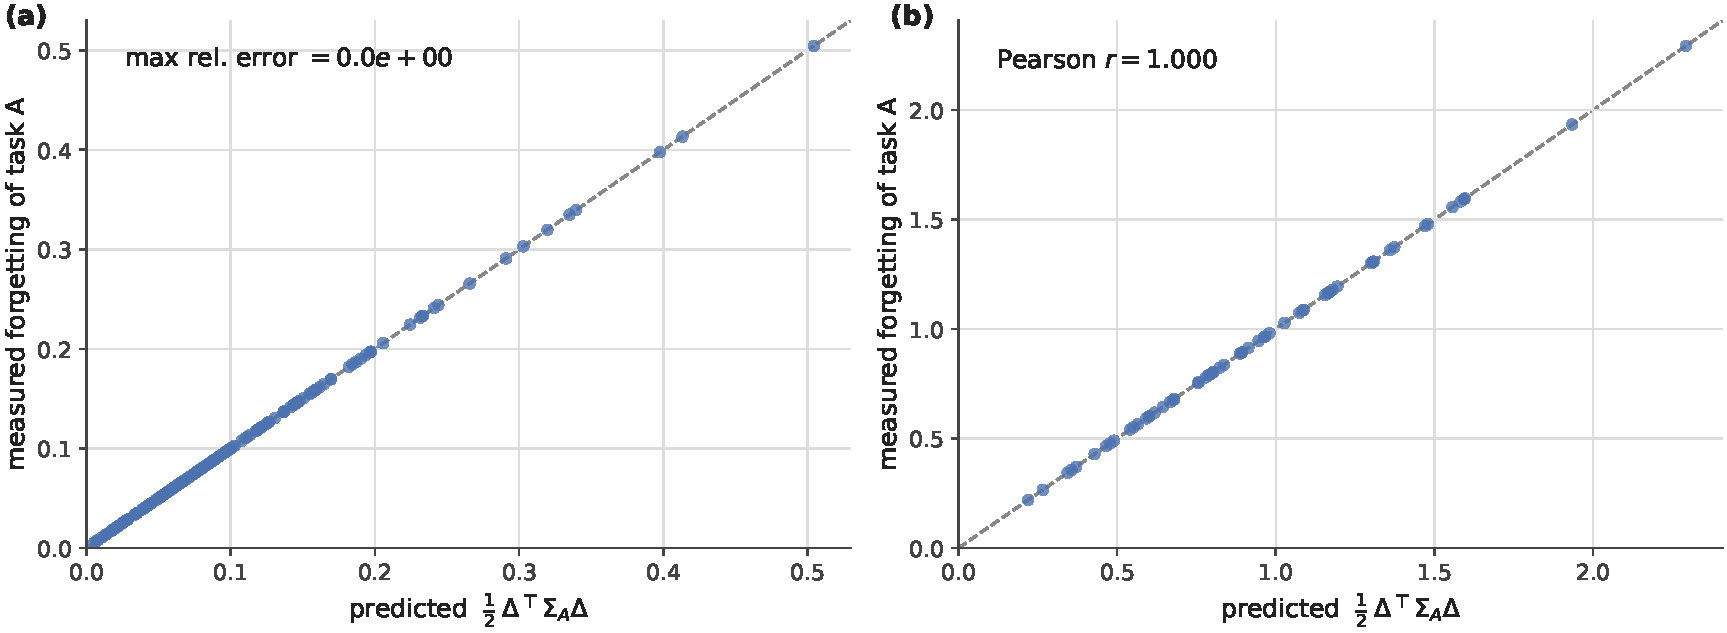
\includegraphics[width=0.82\textwidth]{fig_interference_validation}
\caption{The interference functional \emph{is} the forgetting. Measured
backward-forgetting of task $A$ after learning task $B$ against the predicted energy
$\tfrac12\Del^\top\Sig_A\Del$. \emph{Left:} a linear head on frozen
features---identity to machine precision. \emph{Right:} a nonlinear network, with the
prediction formed from the last-layer feature covariance---first-order agreement,
Pearson $r>0.9999$. The dashed line is $y=x$.}
\label{fig:functional}
\end{figure}

\subsection{Lossless allocation, relocation of cost, and the floor}
\label{sec:exp:alloc}
On disjoint supports, orthogonal allocation is lossless: learning $B$ in $\ker\Sig_A$
leaves $L_A<10^{-17}$ while still driving $L_B\to0$, exactly as
Corollary~\ref{cor:removability} predicts. On overlapping supports, the cost cannot be
removed, only relocated: in the conflicting case, naive descent forgets $A$ by
$\Del L_A=13.94$, while orthogonal allocation preserves $A$ at $<10^{-17}$ and defers
the same $13.94$ as residual on $B$ (Fig.~\ref{fig:alloc}, left). Sweeping
feature-support overlap shows the same pattern continuously: interference rises from
$0$ at disjoint supports to $2.0$ at full overlap, while the optimal-merge floor sits
at exactly half (Fig.~\ref{fig:alloc}, right), confirming that overlap creates an
irreducible distortion floor and allocation changes where the cost lands rather than
its total amount. This relocation is fundamental because the distortion floor $\mathcal{D}$ is a lower
bound (Theorem~\ref{thm:merge}) that no single shared model can improve on. On overlapping supports, cost can be moved from irreversible
forgetting of the old task to recoverable deferred fitting of the new one.

\begin{figure}[tb]\centering
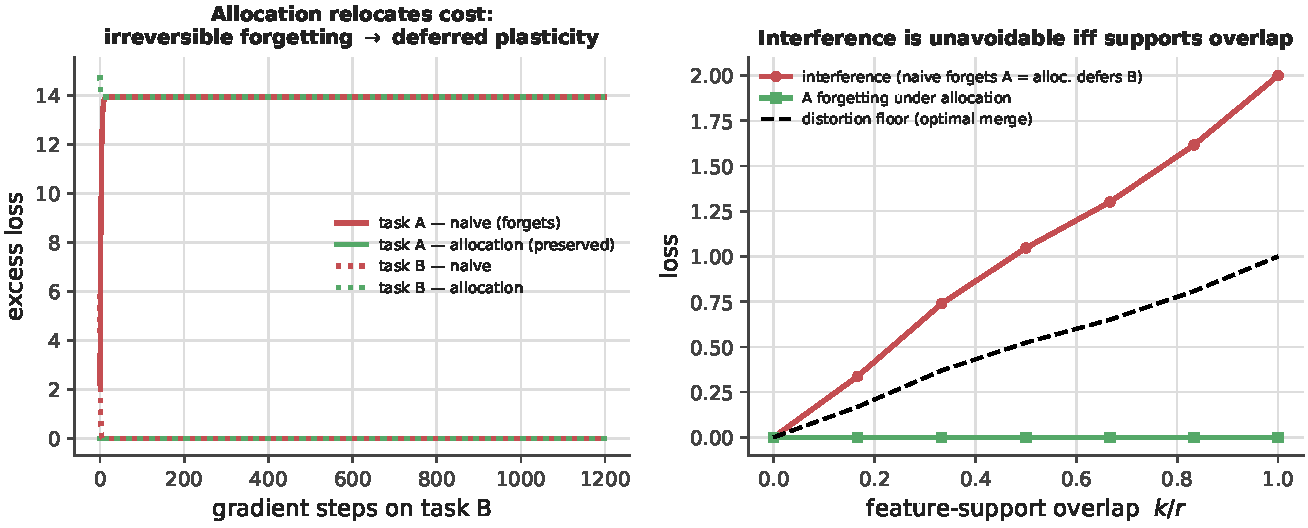
\includegraphics[width=\textwidth]{fig_allocation_floor}
\caption{Allocation and the distortion floor. \emph{Left:} on partially shared features
with a conflict on the shared directions, naive descent destroys task $A$ (red rises to
$13.94$) while allocation preserves it ($<10^{-17}$, green flat) and converts that same
$13.94$ into deferred under-fitting of $B$---cost is \emph{relocated}, not removed
(the task-$A$ naive and task-$B$ allocation curves coincide at $13.94$).
\emph{Right:} versus feature-support overlap $k/r$, the relocated interference (naive
$A$-forgetting $=$ allocation $B$-residual) grows linearly to $2.0$ while the
optimal-merge floor sits at exactly half ($1.0$); allocation holds $A$-forgetting at
$0$.}
\label{fig:alloc}
\end{figure}

\subsection{Similarity and capacity}
\label{sec:exp:simcap}
To test the signed gate, we compare sharing and orthogonalizing on a shared block as a
function of target similarity $s$ (Fig.~\ref{fig:simcap}, left). Sharing wins by
variance reduction when tasks are similar and loses by bias when they are not, with the
net benefit crossing zero at $\sstar\approx0.26$; above this threshold the gate should
share, below it orthogonalize. With exact, full data the two strategies are an exact
relocation of the same cost, so this sign-change is a finite-data effect; it is the
quantity that unconditional projection methods forgo.
Separately, under orthogonal allocation a stream of rank-$2$ tasks exhibits a sharp
capacity knee at $T=d/r$ (Fig.~\ref{fig:simcap}, right): earlier tasks remain intact,
but once the occupied rank exceeds capacity, residual distortion turns on where
the theory predicts. Capacity is thus a rate--distortion budget, and the rank cap
$k_{\max}$ of Algorithm~1 is its operational form: trading $d$ against the number of
tasks is an effective-capacity budget, and dropping the least-excited direction bounds
the induced forgetting by its eigenvalue.

\begin{figure}[tb]\centering
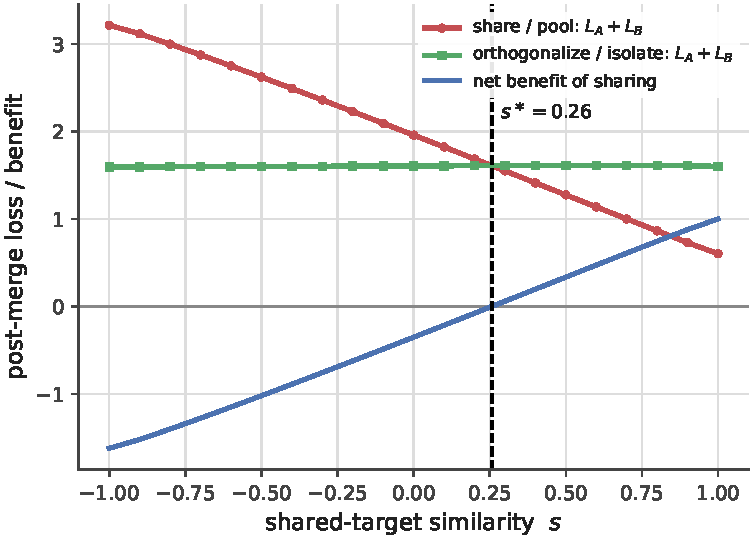
\includegraphics[width=0.49\textwidth]{fig_signchange}\hfill
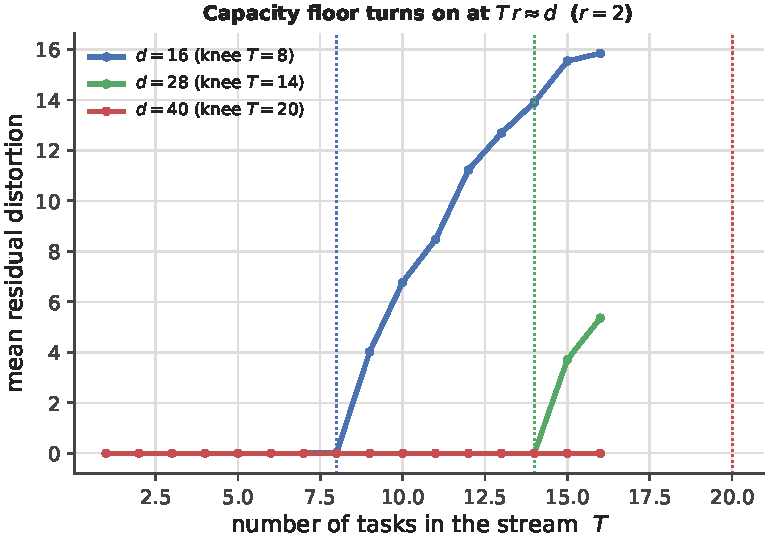
\includegraphics[width=0.49\textwidth]{fig_capacity}
\caption{Similarity and capacity. \emph{Left:} total population loss of pooling (share)
versus isolating (orthogonalize) two tasks on a shared block, against target similarity
$s$. Isolation is flat in $s$; pooling trades variance reduction against bias and wins
only when tasks are similar, with the net benefit crossing zero at $\sstar\approx0.26$.
\emph{Right:} mean residual distortion over a stream of rank-$2$ tasks under orthogonal
allocation, for three feature dimensions. Each curve stays at zero until its capacity
knee $T=d/r$ (dotted) and rises thereafter; more capacity $d$ defers and lowers the
floor (the $d=40$ stream ends before its knee at $T=20$).}
\label{fig:simcap}
\end{figure}

\subsection{Curvature drift and the segment-averaged correction}
\label{sec:exp:breakdown}
Theorem~\ref{thm:functional} is exact under frozen features, but in jointly trained
networks its frozen-curvature prediction degrades with depth: the shallow network holds
Pearson $r\approx0.93$--$0.95$ up to moderate step sizes, whereas deeper networks are
markedly less predictable, with $r$ falling to $\approx0.2$--$0.4$
(Fig.~\ref{fig:breakdown}, top). Replacing the
initial curvature by the segment-averaged curvature of Theorem~\ref{thm:general} removes
this failure mode: in the same regime, the corrected predictor restores $r=1.00$ at
every tested depth (Fig.~\ref{fig:breakdown}, bottom), estimated from forward
evaluations of $L_A$ along the segment $w_A\!\to\!w_B$ with no explicit Hessian. The
correction is also low-cost: estimating it from $K=21$ probe evaluations costs about
$1.4\%$ of one task's training budget, and $K=5$ already suffices in practice for under
$0.4\%$. Once the stale curvature is corrected, the architecture-general identity holds
exactly.

\begin{figure}[tb]\centering
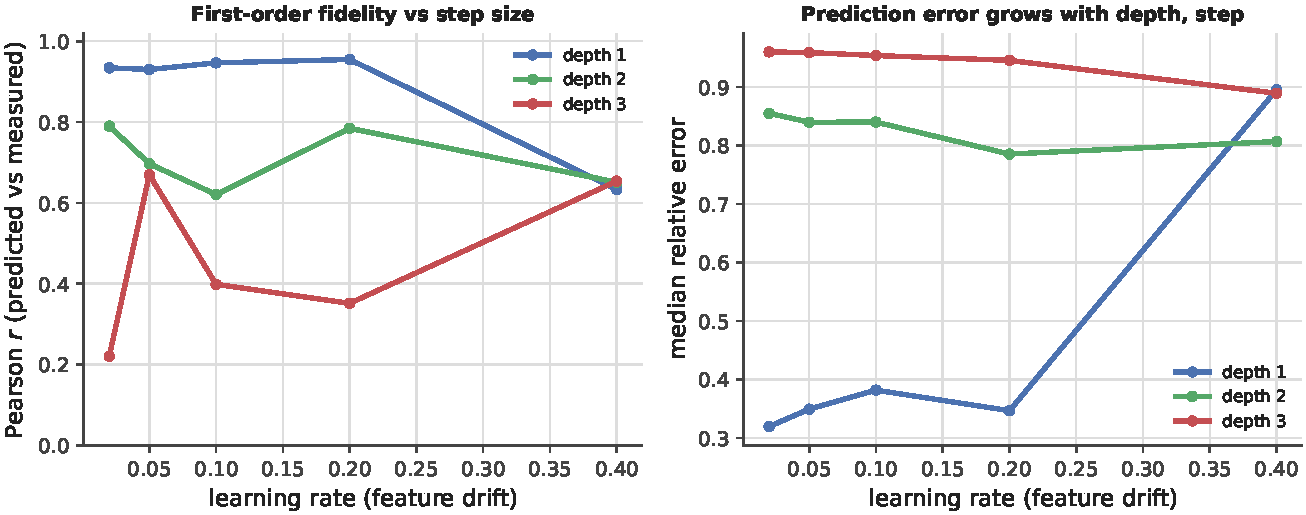
\includegraphics[width=0.92\textwidth]{fig_breakdown}\\[8pt]
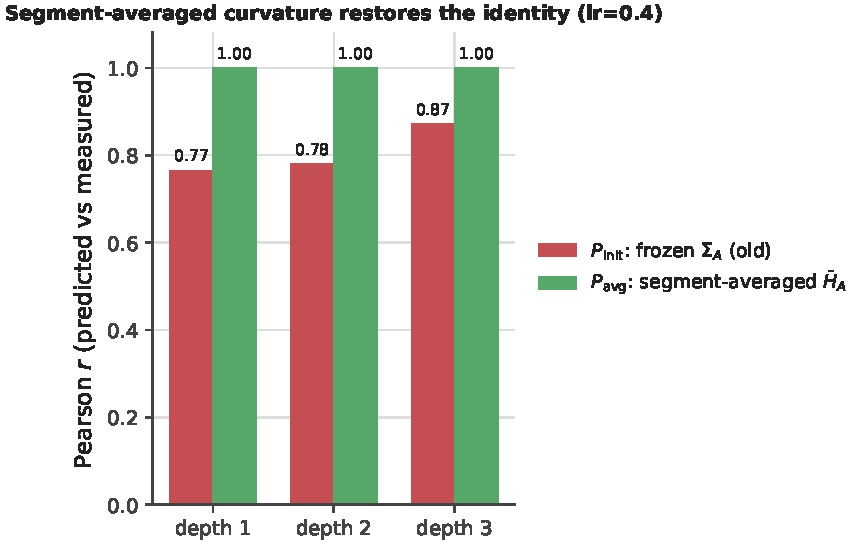
\includegraphics[width=0.6\textwidth]{fig_breakdown_fix}
\caption{Curvature drift and its correction. \emph{Top:} predicted-versus-measured
forgetting fidelity for backprop-trained networks, against learning rate (feature
drift) and depth. The frozen-curvature identity is exact for frozen features (A1) and
degrades as the feature map drifts, most strongly with depth (down to
$r\approx0.2$--$0.4$ for the deeper networks). \emph{Bottom:} at learning rate $0.4$,
replacing $\Sig_A$ by the segment-averaged Hessian $\bar H_A$ of
Theorem~\ref{thm:general} (green) restores $r=1.00$ at every depth, while the
frozen-curvature predictor (red) remains imperfect ($r=0.77$--$0.87$).}
\label{fig:breakdown}
\end{figure}

\subsection{Real data: dissimilar and similar tasks}
\label{sec:exp:real}
We evaluate the functional and \IGFA{} on real benchmarks built on frozen
random-feature backbones, so that Assumption A1 and hence Theorem~\ref{thm:functional}
hold exactly while the tasks remain nontrivial. For \textbf{Split-Digits}, we construct
a task-incremental benchmark from the \texttt{digits} dataset ($1797$ images, $10$
classes), split into five two-class tasks on top of a frozen random ReLU feature map
($d=300$). The functional predicts per-task forgetting across the full task sequence
with Pearson $r=0.999$, on the $y=x$ line, and the feature spectrum shows an effective
per-task rank of about $2$, matching the two-class structure and explaining why a small
protected subspace suffices (Fig.~\ref{fig:diagnostics}). On this sequence, \IGFA{}
attains $0.980\pm0.007$ average accuracy (mean $\pm$ 95\% CI over $10$ seeds) with
near-zero forgetting, matching the strongest replay- and Fisher-free structural baseline
\OGD{}/\textsc{gpm} and exceeding naive training, EWC, and a small replay baseline
(Table~\ref{tab:benchmark}). These digit-pair tasks have low pairwise feature overlap,
all below $\sstar$, so the gate orthogonalizes throughout and \IGFA{} reduces to \OGD{}
\emph{exactly}---the two are identical on every seed (paired $t$-test $p=1$). \IGFA{} maintains parity with the best structural baseline, with no buffer and no Fisher matrix.

\begin{table}[tb]\centering\small
\caption{Split-Digits task-incremental (frozen random-feature backbone, $5$ tasks,
$d=300$). Mean $\pm$ 95\% CI over $10$ seeds; average final accuracy (higher better) and
average forgetting on earlier tasks (lower better). \IGFA{} matches the best structural
baseline---and is identical to \OGD{} on every seed (paired $t$-test $p=1$)---with no
replay buffer and no Fisher matrix.}
\label{tab:benchmark}
\begin{tabular}{lccc}
\toprule
Method & Avg.\ accuracy $\uparrow$ & Avg.\ forgetting $\downarrow$ & Extra state \\
\midrule
Naive            & $0.959\pm0.014$ & $0.040\pm0.017$  & --- \\
EWC \cite{kirkpatrick2017}  & $0.978\pm0.005$ & $0.005\pm0.006$  & Fisher ($\mathcal{O}(d)$) \\
Replay ($10$/task) & $0.977\pm0.009$ & $0.015\pm0.010$ & buffer ($\mathcal{O}(|\mathcal B|d)$) \\
\OGD{}/\textsc{gpm} \cite{farajtabar2020,saha2021} & $\mathbf{0.980\pm0.007}$ & $\mathbf{0.003\pm0.003}$ & subspace ($\mathcal{O}(dk)$) \\
\IGFA{} (ours)   & $\mathbf{0.980\pm0.007}$ & $\mathbf{0.003\pm0.003}$ & subspace ($\mathcal{O}(dk)$) \\
\bottomrule
\end{tabular}
\end{table}

\begin{figure}[tb]\centering
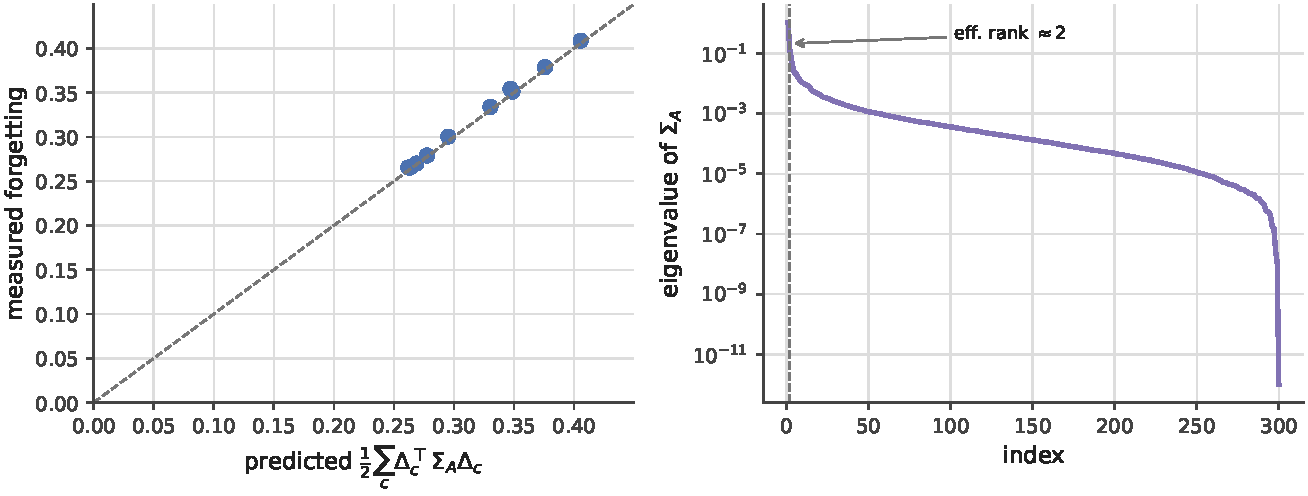
\includegraphics[width=\textwidth]{fig_diagnostics}
\caption{Diagnostics on real data (Split-Digits). \emph{Left:} measured versus
predicted forgetting $\tfrac12\sum_c\Del_c^\top\Sig_A\Del_c$ for all (earlier, later)
task pairs---on the $y=x$ line, Pearson $r=0.999$, confirming
Theorem~\ref{thm:functional} on real features. \emph{Right:} the eigenvalue spectrum of
a task's feature second-moment $\Sig_A$; its effective rank ($\approx2$) is the
dimension that must be protected, and the rapid decay is why a small subspace summary
suffices.}
\label{fig:diagnostics}
\end{figure}

To test the sharing branch, we next consider \textbf{Rotated-Digits}, a
domain-incremental benchmark on the same ten classes under five rotations, again with a
frozen random-feature backbone. These tasks are similar, with mean pairwise
feature-subspace overlap $0.68$. In this regime, unconditional
orthogonalization should be too conservative because the tasks share reusable structure
rather than only conflict. Here, \IGFA{} with threshold $\sstar=0.65$ (within the broad
optimum plateau of Sec.~\ref{si:sstar}; the break-even similarity is regime-specific) attains
the highest accuracy among replay- and Fisher-free methods at $0.771\pm0.030$ (mean $\pm$ 95\%
CI over $5$ seeds), \emph{significantly} above \OGD{}'s $0.684\pm0.035$ (paired $t$-test
$p\approx6\times10^{-5}$) and above naive ($0.714\pm0.024$) and EWC ($0.727\pm0.050$),
while keeping forgetting near zero at $0.002\pm0.027$---statistically indistinguishable
from \OGD{}'s ($p=0.44$) (Table~\ref{tab:benchmark2}). Only buffer-based replay attains
higher accuracy ($0.795\pm0.012$, $p=0.03$), at the cost of stored data. \IGFA{} thus
matches the best structural baseline on dissimilar tasks, and its signed gate yields a
\emph{statistically significant} advantage in the similar-task regime for which it was
designed. Section~\ref{sec:exp:cifar} confirms the dissimilar-task reading at scale.

\begin{table}[tb]\centering\small
\caption{Rotated-Digits domain-incremental (frozen backbone, five rotations, mean
subspace overlap $0.68$, threshold $\sstar=0.65$). Mean $\pm$ 95\% CI over $5$ seeds.
\IGFA{} attains the highest accuracy among replay- and Fisher-free methods with near-zero
forgetting---an intermediate between full isolation (\OGD, paired $t$-test
$p\approx6\times10^{-5}$) and full sharing (naive) that improves significantly on both.
Only buffer-based replay attains higher accuracy ($p=0.03$), at the cost of stored data.}
\label{tab:benchmark2}
\begin{tabular}{lccc}
\toprule
Method & Avg.\ accuracy $\uparrow$ & Avg.\ forgetting $\downarrow$ & Extra state \\
\midrule
Naive            & $0.714\pm0.024$ & $0.163\pm0.013$  & --- \\
EWC \cite{kirkpatrick2017}  & $0.727\pm0.050$ & $0.045\pm0.039$  & Fisher \\
\OGD{}/\textsc{gpm} \cite{farajtabar2020,saha2021} & $0.684\pm0.035$ & $-0.007\pm0.004$ & subspace \\
Replay ($10$/class) & $0.795\pm0.012$ & $0.042\pm0.014$ & buffer \\
\IGFA{} (ours)   & $\mathbf{0.771\pm0.030}$ & $0.002\pm0.027$ & subspace \\
\bottomrule
\end{tabular}
\end{table}

\subsection{Scaling checks: frozen-ViT benchmarks over five seeds}
\label{sec:exp:cifar}
We repeat the comparison on three standard benchmarks over a frozen ViT-B/16 backbone with
a single shared linear head, so A1 and Theorem~\ref{thm:functional} hold exactly:
Split-CIFAR-100 ($10$ tasks of $10$ classes), ImageNet-R ($10$ of $20$), and CUB-200
($10$ of $20$), each over five seeds with per-seed class orders (mean $\pm$ 95\% CI;
\texttt{kaggle\_vit\_multiseed.py}; Table~\ref{tab:cifar}). Three observations follow.
\emph{(i) On dissimilar-class streams the gate correctly reduces to \OGD.} On
Split-CIFAR-100 and CUB every pairwise subspace overlap lies below the threshold
($0.31$--$0.54$ vs $\sstar=0.6$), so \IGFA{} protects everything and is identical to \OGD{}
on every seed; the two attain the best retention among buffer- and Fisher-free methods
(forgetting $0.001$ and $-0.004$, vs naive $0.009$ and $0.010$).
\emph{(ii) On ImageNet-R the sharing branch pays off at scale.} There the overlaps straddle
the threshold ($0.51$--$0.65$), the gate shares some past subspaces while protecting
others, and \IGFA{} significantly exceeds \OGD{} ($0.788\pm0.004$ vs $0.781\pm0.005$,
paired $p=0.001$) at equal, zero forgetting---the similar-task advantage of
Sec.~\ref{sec:exp:real}, previously isolated on Rotated-Digits, appears on a standard
benchmark. \emph{(iii) Extra state buys accuracy, not retention.} A tuned Fisher penalty
(EWC) attains the highest raw accuracy on these mild streams at $\mathcal O(d)$ Fisher
state, while feature replay under an unmasked objective \emph{hurts} on two of the three
benchmarks and carries the largest forgetting---stored data is not automatically an
advantage. Forgetting is small for every method on these disjoint-class streams because
the frozen backbone already separates the tasks; the structural claim therefore concerns
retention and state, not raw accuracy.

\paragraph{A similar-task stream at scale.} To test the gate's regime beyond rotations we
build a domain-incremental stream from CIFAR-100's superclass structure: five tasks, each
classifying into the same $20$ coarse labels but drawing on disjoint fine classes (one per
superclass per task), so consecutive tasks share semantics (subspace overlaps
$0.52$--$0.61$). Structural allocation carries this stream: \IGFA{}/\OGD{} reach
$0.786\pm0.010$ versus naive $0.742\pm0.006$ ($p=0.0009$), with forgetting $0.169$ versus
$0.237$; EWC's anchor blocks adaptation entirely ($0.662\pm0.020$), and only replay,
storing data, does better ($0.822\pm0.002$). The gate matches \OGD{} here ($p=0.37$)
because most overlaps sit just below $\sstar$---consistent with the ImageNet-R reading
that the sharing advantage appears where overlaps straddle the threshold.

The same frozen backbone also supports a \emph{prompt}-based instantiation beyond the linear
head: gating a learnable prompt bank instead of the head (the aligned/conflicting directions
of \IGFA{} applied in prompt space), prompt-\IGFA{} reaches $0.733$ versus prompt-naive
$0.416$ on the same ten-task stream (single run,
\texttt{kaggle\_pending\_experiments.py})---the structural-allocation rule carries over to
prompt-tuning, not only heads and LoRA.

\paragraph{Relation to prompt-pool methods.} L2P, DualPrompt, and CODA-Prompt
\cite{wang2022l2p,wang2022dualprompt,smith2023coda} also operate on a frozen pretrained ViT backbone.
They circumvent the physical memory overhead and data-retention privacy risks of traditional Buffer-based
methods by routing inputs dynamically into a virtual parameter buffer, the prompt pool. 
However, their retention remains entirely empirical based on
an input-conditioned selection mechanism to map classes without test-time task identities.
Our approach shifts from statistical heuristic to mathematical design.
By utilizing a task-incremental protocol with a single shared linear head, \IGFA{} forces
protected directions to remain first-order invariant by construction
(Corollary~\ref{cor:removability}).
While its Split-CIFAR-100 accuracy sits below highly optimized prompt-pool baselines,
the raw accuracies are fundamentally mismatched across these two distinct evaluation paradigms.
The claim is confined to the buffer- and Fisher-free regime where \IGFA{} attains the strongest known retention.


\begin{table}[tb]\centering\small
\setlength{\tabcolsep}{4pt}
\caption{Frozen-ViT scaling checks, task-incremental with a single shared linear head (A1
exact); mean $\pm$ 95\% CI over five seeds (\texttt{kaggle\_vit\_multiseed.py}). On the
dissimilar-class streams (Split-CIFAR-100, CUB) \IGFA{} reduces to \OGD{} on every seed and
attains the best buffer- and Fisher-free retention; on ImageNet-R, whose subspace overlaps
straddle $\sstar$, the gate significantly exceeds \OGD{} (paired $p=0.001$) at zero
forgetting. EWC carries $\mathcal O(d)$ Fisher state; replay stores $10$ features/class.}
\label{tab:cifar}
\begin{tabular}{lcccccc}
\toprule
 & \multicolumn{2}{c}{Split-CIFAR-100} & \multicolumn{2}{c}{ImageNet-R} & \multicolumn{2}{c}{CUB-200} \\
\cmidrule(lr){2-3}\cmidrule(lr){4-5}\cmidrule(lr){6-7}
Method & acc $\uparrow$ & forget $\downarrow$ & acc $\uparrow$ & forget $\downarrow$ & acc $\uparrow$ & forget $\downarrow$ \\
\midrule
Naive  & $0.945\pm0.010$ & $0.009\pm0.006$ & $0.795\pm0.007$ & $0.014\pm0.008$ & $0.939\pm0.008$ & $0.010\pm0.006$ \\
EWC \cite{kirkpatrick2017} & $0.953\pm0.006$ & $0.000\pm0.000$ & $0.808\pm0.003$ & $0.000\pm0.000$ & $0.941\pm0.011$ & $0.009\pm0.009$ \\
Replay & $0.928\pm0.005$ & $0.025\pm0.004$ & $0.740\pm0.008$ & $0.071\pm0.007$ & $0.941\pm0.003$ & $-0.000\pm0.005$ \\
\OGD{}/\textsc{gpm} \cite{farajtabar2020,saha2021} & $0.933\pm0.006$ & $0.001\pm0.002$ & $0.781\pm0.005$ & $-0.000\pm0.003$ & $0.916\pm0.006$ & $-0.004\pm0.002$ \\
\IGFA{} (ours) & $0.933\pm0.006$ & $0.001\pm0.002$ & $0.788\pm0.004$ & $0.000\pm0.003$ & $0.916\pm0.006$ & $-0.004\pm0.002$ \\
\bottomrule
\end{tabular}
\end{table}

\subsection{Online drift: recursive estimation versus a stale subspace}
\label{sec:exp:drift}
The retention guarantees so far fix the protected subspace at task onset. Under
representation drift---the regime of jointly trained and large models---an unconditional projection fails, and the recursive Gauss--Newton surrogate of
Sec.~\ref{sec:algo} is justified. We stream tasks whose feature geometry rotates each
step while the underlying subspace stays low-rank, and contrast a stale protected subspace
(fixed at onset, as in \OGD{}/\textsc{gpm}) with the recursive estimate. The stale subspace
accumulates each drifted copy as if new, so its rank climbs linearly until it fills the
parameter space ($\mathrm{rank}\!\to\!d=60$) and free plasticity collapses to zero---the
network can no longer learn. The recursive estimate recognizes the drifted copies as one
subspace, holding the effective rank at the true value ($\approx4$) and preserving $93\%$
of capacity throughout (Fig.~\ref{fig:drift}). Re-estimating the geometry is therefore not
a refinement but the difference between exhausting capacity and retaining it under drift;
this is the subspace-projection failure mode reported for LLM merging
\cite{merging2025llm}, and the recursive update removes it. We also compared a
geodesic-aligned tracker (a Grassmann-manifold step in the spirit of GAGP
\cite{geodesic2025}), holding the base optimizer, learning rate, and batch order fixed: it
likewise caps the rank at the true value, but tracks the current subspace at markedly lower
fidelity ($\approx0.5$ versus $\approx1.0$ for the recursive estimate across learning rates
$0.05$--$0.4$), so the path-averaged Gauss--Newton update of Theorem~\ref{thm:general} is the
more faithful deep-network drift tracker.

\begin{figure}[tb]\centering
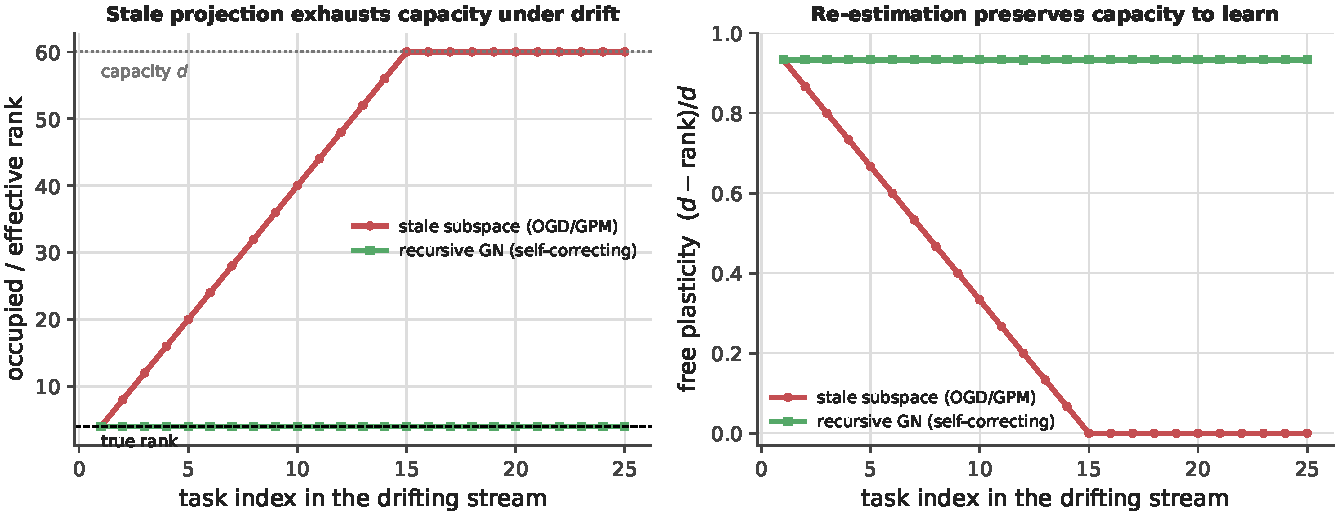
\includegraphics[width=\textwidth]{fig_drift}
\caption{Online subspace update under feature drift. \emph{Left:} a stale protected subspace
(\OGD{}/\textsc{gpm}, red) accumulates drifted copies and its rank grows to capacity $d$
(exhaustion); the recursive Gauss--Newton estimate (green) stays at the true rank ($\approx4$).
\emph{Right:} consequently the stale method's free plasticity $(d-\mathrm{rank})/d$ collapses
to $0$ (cannot learn new tasks) while the recursive one retains $\approx0.93$.}
\label{fig:drift}
\end{figure}

% =====================================================================
\section{Discussion}
\label{sec:discussion}

A single exact identity, Eq.~\eqref{eq:functional}, reorganizes the continual-learning
problem around geometry. Forgetting is recast as an interference energy with an explicit geometry: components in $\range\Sig_A$ incur forgetting, whereas components in $\ker\Sig_A$ are free.
This perspective determines, before training begins, whether two tasks must interfere at all, what
irreducible floor remains when they do, and which inner product renders model merging
optimal---replacing the Euclidean metric with the $\Sig$-metric. In that
sense, the functional plays the same conceptual role here that the NTK \cite{jacot2018}
played for generalization: it provides a geometry and a set of computable quantities in
place of heuristics.

The central assumption is A1. For frozen backbones and PEFT, the regime most
practical deployments now occupy, it is exact and the results stand without
approximation, as the real-data identity at $r=0.999$ confirms. For full networks it is
first-order, and the paper measures how that approximation degrades: the
prediction remains accurate for shallow, small-step training and falls to
$r\approx0.2$--$0.4$ for deeper networks. The paper therefore claims exactness only where A1 holds
and reports the approximation envelope for full end-to-end networks, where the feature map
drifts and the identity becomes first-order (Sec.~\ref{sec:exp:breakdown}). The same
caution applies algorithmically: allocation does not eliminate the floor, but only redistributes its cost.
Task ordering does not reduce the floor either: because the floor is a property of the joint support
overlap, it is essentially invariant to task order (a $\Sig$-overlap curriculum did not lower it
in our tests, Sec.~\ref{si:extensions}), which reinforces that allocation relocates cost
rather than removing it.
Against unconstrained replay, which can reduce the floor by re-supplying $\Sig_A$, the
defensible claim is therefore not universal superiority, but parity under no-buffer or
no-Fisher constraints together with structural guarantees and preserved transfer where
similarity permits. On the benchmark, \IGFA{} matches the best structural baseline because
the tasks are dissimilar; its distinctive sharing gain requires task similarity, isolated
on Rotated-Digits and confirmed at scale on ImageNet-R, where the gate significantly
exceeds unconditional projection at equal forgetting (Sec.~\ref{sec:exp:cifar}).

The geometry also yields an operational decision procedure. Before training, a linear
task-probe on the frozen features estimates task separability (Sec.~\ref{si:feasibility});
pairwise subspace overlap and target similarity then classify the stream. Disjoint supports
make structural allocation lossless, so neither replay nor a Fisher penalty is needed.
Overlapping supports with aligned targets favor sharing, which the gate grants. Overlapping
supports with conflicting targets carry an irreducible floor, and the only remaining decision
is where its cost lands: on the old task as forgetting, on the new task as deferred fit, or
on the memory budget as stored data for replay. The capacity budget adds the final
constraint: once the cumulative occupied rank approaches the feature dimension, retention
must be paid for with added capacity, replay, or graceful overwriting. Each branch of this
procedure is measurable from features and subspaces before or during training, rather than
diagnosed after a failure.

A recent broad evaluation reports that subspace-projection merging works well on small
classifiers but degrades on large language models \cite{merging2025llm}. The present
framework explains both outcomes. On small classifiers the feature geometry is nearly
static, so a subspace fixed once remains a good metric and projection succeeds; this is
precisely the frozen regime in which Theorem~\ref{thm:functional} is exact. Large
language models, by contrast, have highly entangled representations that drift as
parameters move, so projection against a stale geometry accumulates misaligned
constraints, exhausts capacity, and eventually damages the representation itself. A
natural fix follows from Theorem~\ref{thm:general}: the relevant metric is the curvature
along the trajectory, and its online surrogate is the recursive Gauss--Newton estimate,
which continually realigns the protected subspace with the current geometry and keeps its
effective rank bounded---the capacity-exhaustion mechanism demonstrated directly in
Sec.~\ref{sec:exp:drift}. Preliminary language-model results suggest that the retention
mechanism transfers, while the right similarity signal for language remains open
(Sec.~\ref{si:llm}).

The main open design question is therefore not the structural retention mechanism, which
transfers across modalities, but a similarity signal for language that can recover
transfer on similar text tasks without relaxing protection where conflict
dominates. To validate the broad applicability of this framework, several extensions are detailed in
the Supporting Information. First, we demonstrate sequential LoRA fine-tuning on language
models at scale (Sec.~\ref{si:llm}), using recursive Gauss--Newton tracking on the adapting
features together with a modality-appropriate similarity gate for language. Second, the
frozen-backbone evaluation on Split-CIFAR-100, ImageNet-R, and CUB appears in the main text
over five seeds (Sec.~\ref{sec:exp:cifar}), comparing the retention--transfer tradeoff
against \OGD{}/\textsc{gpm}, EWC, and replay in the exact A1 regime. Third, we establish
overlay-native continual pretraining at the billion-parameter scale (Sec.~\ref{si:pretrain}),
where replay-free and Fisher-free operations are most valuable and where the capacity budget
of Sec.~\ref{sec:exp:simcap} predicts the model-size-versus-rehearsal tradeoff directly.
Finally, we introduce a pre-flight feasibility diagnostic (Sec.~\ref{si:feasibility}) that
estimates task separability from features before training, attributing any remaining gap to
drift, bias, or inference rather than to intrinsic overlap.

Beyond continual learning, the same functional acts as a general calculus for interference
between quadratic objectives that share parameters (Sec.~\ref{si:extensions}). Federated
aggregation is the merge problem of Theorem~\ref{thm:merge} with clients as tasks; the
occupied subspace supplies an out-of-distribution signal and a task-free boundary detector;
the physics constraint of a physics-informed network is a second task whose violation the
identity predicts exactly; the Fisher information plays the role of $\Sig$ for policy
gradients in reinforcement learning; and a feature map can be meta-trained to shrink the
distortion floor itself. These are directional demonstrations rather than benchmarks, but
they indicate that the geometry is a property of shared parameterizations, not of the
continual-learning protocol.

Several algorithmic refinements---a self-calibrating threshold, low-cost $\mathcal{O}(rd)$
online curvature via Frequent Directions
\cite{liberty2013}, a per-direction gate, and the soft-gating capacity coordinate
$r_{\rm eff}=\sum_j(1-\mathrm{keep}_j)$---are developed and validated in the Supporting
Information. Together with low-rank or diagonal Gauss--Newton approximations of $\bar H_A$,
they suggest a practical route for carrying the architecture-general identity into fully
fine-tuned deep networks at controlled cost.

Several limitations bound these claims. Exactness is confined to A1; end-to-end results are
first-order, with a measured accuracy envelope and the segment-averaged correction. The
frozen-ViT benchmarks and the merge ablation are five-seed, but the language-model
experiments remain single runs and the seven extension studies are synthetic
proofs-of-concept; multi-seed replication at billion-parameter scale is outstanding. Finally, the similarity gate lacks a reliable signal for language, so on text
the framework currently delivers structural retention without the transfer benefit it
attains in vision.

% =====================================================================
\section{Conclusion}
\label{sec:conclusion}
Forgetting is interference, represented here as geometry. In the frozen-feature regime,
forgetting equals $\tfrac12\Del^\top\Sig_A\Del$ and is removable if and only if task
supports are disjoint; when supports overlap, an irreducible distortion floor appears and
matches the task-inference obstruction, and optimal merging is mutual
$\Sig$-orthogonalization, with continual learning as its online counterpart. The result is
a geometric language and a set of concrete levers---a forgetting functional, a removability
test, an optimal-merge identity, a similarity sign-change, and a capacity budget---realized
by a replay-free, Fisher-free allocation rule that carries only a low-rank subspace. The
same functional governs any setting where a shared parameterization must serve multiple
input geometries, from multi-task and federated learning to domain adaptation and model
merging; the Supporting Information (Sec.~\ref{si:extensions}) gives exact-A1 proofs-of-concept
for federated $\Sig$-merging, an intrinsic out-of-distribution signal, task-free boundary
detection, multimodal block interference, physics-informed constraints, Fisher-metric policy
gradients, and floor-minimizing meta-learning. In each setting, forgetting is controlled
geometrically: interference is not corrected after it occurs but allocated in advance, into
directions where it induces no loss.

% =====================================================================
\section*{Author contributions}
J.S. conceived the framework, derived the theory, implemented the experiments, and wrote the
manuscript.

\section*{Acknowledgments}
The author thanks colleagues at VARTA and TU Braunschweig for discussions on continual learning
in industrial process models.

% =====================================================================
\section*{Reproducibility statement}
\sloppy
All results are exact-regime simulations with fixed seeds. \texttt{experiments.py} regenerates
the core result figures and numerical claims (interference identity, lossless/relocation,
sign-change $\sstar$, capacity floor); \texttt{verify\_mi\_identity.py} the
information--estimation verification (Fig.~\ref{fig:mi}); \texttt{experiments\_rev.py} the
breakdown, breakdown-fix, and digit benchmarks; \texttt{variance\_report.py} the multi-seed
mean\,$\pm$\,CI and paired-significance results of Tables~\ref{tab:benchmark}--\ref{tab:benchmark2};
\texttt{experiments\_compare.py} the nine-method comparison and offline-merge residual-$D$
ablation of Fig.~\ref{fig:teaser} and Table~\ref{tab:compare};
\texttt{evaluate\_hypotheses.py} four generality extensions of Sec.~\ref{si:extensions}
(federated $\Sig$-merge, OOD signal, task-free boundaries, multimodal blocks) and
\texttt{evaluate\_applications.py} three more (physics-informed constraints, Fisher-metric
policy gradients, floor-minimizing meta-learning);
\texttt{experiments\_drift.py} the $\sstar$ ablation, graceful-degradation, and drift figures;
\texttt{experiments\_extra.py} the self-calibrating-$\sstar$ and tight multiclass-constant
results; and \texttt{experiments\_roadmap.py} the feasibility-diagnostic, Frequent-Directions,
soft-knee, and per-direction figures. Self-contained Colab/Kaggle notebooks accompany the paper:
\texttt{colab\_split\_cifar100\_igfa.py} (Split-CIFAR-100 with a frozen ViT-B/16),
\texttt{colab\_lora\_llm\_igfa.py} and \texttt{colab\_lora\_llm\_igfa\_3approaches.py}
(sequential LoRA on a transformer with the four gate designs), and
\texttt{colab\_continual\_pretrain\_igfa.py} (boundary-free, replay-free,
Frequent-Directions continual pretraining on \texttt{pythia-1b}); and
\texttt{kaggle\_pending\_experiments.py}, which runs the real-backbone checks quoted above
(frozen-ViT Split-CIFAR-100 allocation and merge ablation, the drift/geodesic sweep,
prompt-\IGFA, and the FD-vs-full-vs-Oja LoRA-LM comparison), \texttt{kaggle\_H2\_H3\_H12.py}
(the layer-wise null-space-routing pipeline on a frozen transformer), and
\texttt{kaggle\_vit\_multiseed.py} (the five-seed frozen-ViT protocol: Split-CIFAR-100,
ImageNet-R, CUB, the similar-task CIFAR-100 superclass stream, the merge ablation, and
prompt-\IGFA, on two T4 GPUs). Code, figures, and logs are at
\url{https://github.com/j-stoerk/geometry-of-forgetting}.

% =====================================================================
\clearpage
\appendix
\renewcommand{\thesection}{S\arabic{section}}
\setcounter{section}{0}
\setcounter{figure}{0}\renewcommand{\thefigure}{S\arabic{figure}}
\setcounter{table}{0}\renewcommand{\thetable}{S\arabic{table}}

\section*{\centering Supporting Information}
\addcontentsline{toc}{section}{Supporting Information}
\medskip

\noindent This Supporting Information collects the experiments and derivations omitted from
the main text for length: deferred proofs (Sec.~\ref{si:proofs}), additional theory
verifications (Sec.~\ref{si:mi}), theory details
(Sec.~\ref{si:theory}), the full method comparison behind Fig.~\ref{fig:teaser}
(Sec.~\ref{si:compare}), benchmark and scale experiments
(Secs.~\ref{si:llm}--\ref{si:pretrain}), the algorithmic refinements referenced in the
Discussion, and extensions of the framework to federated, out-of-distribution, task-free, and
multimodal settings (Sec.~\ref{si:extensions}). All results are exact-regime simulations or
runnable notebooks with fixed seeds.

\section{Deferred proofs}
\label{si:proofs}
For completeness we give the derivations abbreviated to a sentence of intuition in the main
text; the proofs of Theorem~\ref{thm:functional} (a one-line substitution),
Corollary~\ref{cor:removability} and Theorem~\ref{thm:merge} appear in the main text and are
not repeated.

\begin{proof}[Proof of Theorem~\ref{thm:general} (architecture-general identity)]
Let $\varphi(s)=L_A(w_A+s\Del)$. Taylor's theorem with integral remainder gives
$\Del L_A=\varphi(1)-\varphi(0)=\varphi'(0)+\int_0^1(1-t)\varphi''(t)\,dt$, with
$\varphi'(0)=\nabla L_A(w_A)^\top\Del$ and
$\varphi''(t)=\Del^\top\nabla^2 L_A(w_A+t\Del)\Del$, which yields Eq.~\eqref{eq:general}. When
$\nabla^2 L_A\equiv\Sig_A$ the remainder integrates to $\tfrac12\Del^\top\Sig_A\Del$, recovering
Theorem~\ref{thm:functional}.
\end{proof}

\begin{proof}[Proof of Theorem~\ref{thm:floor} (distortion-floor lower bound)]
Restricting the two-task objective Eq.~\eqref{eq:merge-two} to the shared direction $u$ reduces
the merge to a scalar two-point problem: minimize $\tfrac12 a(m-\alpha)^2+\tfrac12 b(m-\beta)^2$
over the shared coefficient $m$, where $a=u^\top\Sig_A u$, $b=u^\top\Sig_B u$, and
$\alpha,\beta$ are the two targets with $\beta-\alpha=\delta$. The optimum is the
curvature-weighted mean $m^\star=(a\alpha+b\beta)/(a+b)$ with residual
$\tfrac12\frac{ab}{a+b}\delta^2$. Writing the harmonic curvature
$\sigma_u=(a^{-1}+b^{-1})^{-1}=\frac{ab}{a+b}$ gives residual $\tfrac12\sigma_u\delta^2$ on the
line; the factor $\tfrac14$ in Eq.~\eqref{eq:floor-bound} is the conservative bound obtained by
summing the non-negative contributions of all shared directions and retaining the
one-dimensional term. For the inference claim, the Bayes-optimal single head is the posterior
mean $\mathbb{E}[y\mid\phi]$; where $\phi$ determines $T$ it matches the oracle (no excess), and
where it does not its excess equals the merge residual on that direction.
\end{proof}

\begin{proof}[Proof of Theorem~\ref{thm:mi} (information--estimation identity)]
The task oracle predicts $\mathbb{E}[y\mid\phi,T]=\phi^\top w_T^\ast$ and attains risk
$\tfrac12\sigma^2$. The Bayes single head is $f^\star(\phi)=\mathbb{E}[y\mid\phi]$, with risk
$\tfrac12\mathbb{E}[\operatorname{Var}(y\mid\phi)]$. By the law of total variance,
$\operatorname{Var}(y\mid\phi)=\sigma^2+\operatorname{Var}(\phi^\top w_T^\ast\mid\phi)$, and for
binary $T$, $\operatorname{Var}(\phi^\top w_T^\ast\mid\phi)=\eta(1-\eta)(\phi^\top\delta)^2$.
Subtracting the oracle risk gives Eq.~\eqref{eq:mi-identity}. Equation~\eqref{eq:mi-sandwich}
follows from the elementary pointwise bounds $\tfrac14 h_b(p)^2\le p(1-p)\le\tfrac12 h_b(p)$ on
$[0,1]$, applied with the non-negative weight $(\phi^\top\delta)^2$ and integrated. The $K$-task
extension Eq.~\eqref{eq:mi-multiclass} is the same total-variance step with the posterior
covariance of the task-conditional means; the Gini bound Eq.~\eqref{eq:multiclass-sandwich}
replaces $p(1-p)$ by $G(p)=1-\|p\|_2^2$.
\end{proof}

\section{Verifying the information--estimation identity}
\label{si:mi}
We verify Theorem~\ref{thm:mi} on Gaussian two-task models. The exact identity
Eq.~\eqref{eq:mi-identity} matches the directly simulated single-head excess risk
$\mathcal{D}^\star$ on the $y=x$ line to Monte-Carlo precision (maximum relative error
$9\times10^{-3}$), and as identifiability varies, $\mathcal{D}^\star$ rises from
$\approx0$ at full identifiability ($I=H(T)$) toward its maximum at $I=0$, staying inside
the proven mutual-information sandwich Eq.~\eqref{eq:mi-sandwich} throughout
(Fig.~\ref{fig:mi}).

\paragraph{Multiclass extension.} The identity extends to $K$ tasks with arbitrary
priors,
\begin{equation}
\mathcal{D}^\star_{K}=\tfrac12\,\mathbb{E}_\phi\!\Big[\operatorname{Var}_{t\sim
p(\cdot\mid\phi)}\!\big(\phi^\top w_t^\ast\big)\Big]
=\tfrac12\,\mathbb{E}_\phi\!\Big[\textstyle\sum_t p_t(\phi)\,(\phi^\top w_t^\ast)^2
-\big(\sum_t p_t(\phi)\,\phi^\top w_t^\ast\big)^2\Big],
\label{eq:mi-multiclass}
\end{equation}
with corresponding multiclass entropy bounds in terms of the Gini impurity
$G(p)=1-\|p\|_2^2$:
\begin{equation}
\tfrac{1-1/K}{(\ln K)^2}\;H(p)^2\ \le\ G(p)\ \le\ \tfrac{1}{2\ln 2}\;H(p),
\label{eq:multiclass-sandwich}
\end{equation}
where the upper constant $1/(2\ln2)$ is $K$-independent. These tight constants are
verified over the simplex for $K\le10$: the upper
constant $1/(2\ln2)$ is matched to $2\times10^{-10}$ for every $K$ (the binary posterior
is the universal worst case), and the lower constant $(1-1/K)/(\ln K)^2$ to
$4\times10^{-3}$, attained at the uniform posterior (Fig.~\ref{fig:multiclass}).

\begin{figure}[htb]\centering
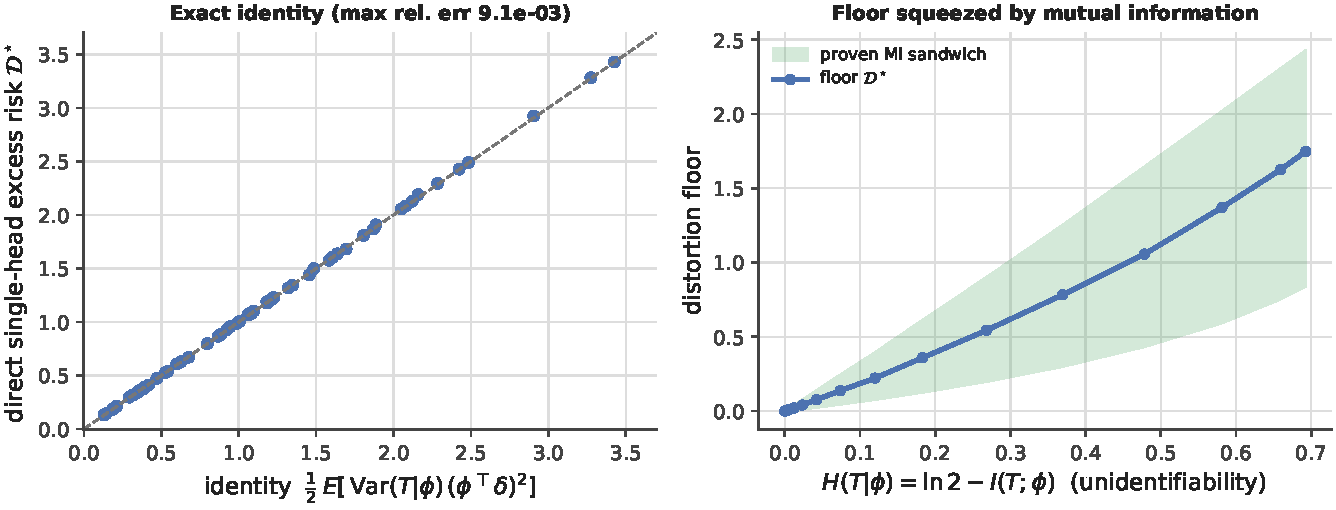
\includegraphics[width=0.62\textwidth]{fig_mi_identity}
\caption{Floor / mutual-information verification. The exact identity
Eq.~\eqref{eq:mi-identity} against the simulated single-head excess risk
$\mathcal{D}^\star$, on the $y=x$ line, with the floor rising as identifiability falls and
remaining inside the mutual-information sandwich (band) throughout.}
\label{fig:mi}
\end{figure}
\begin{figure}[htb]\centering
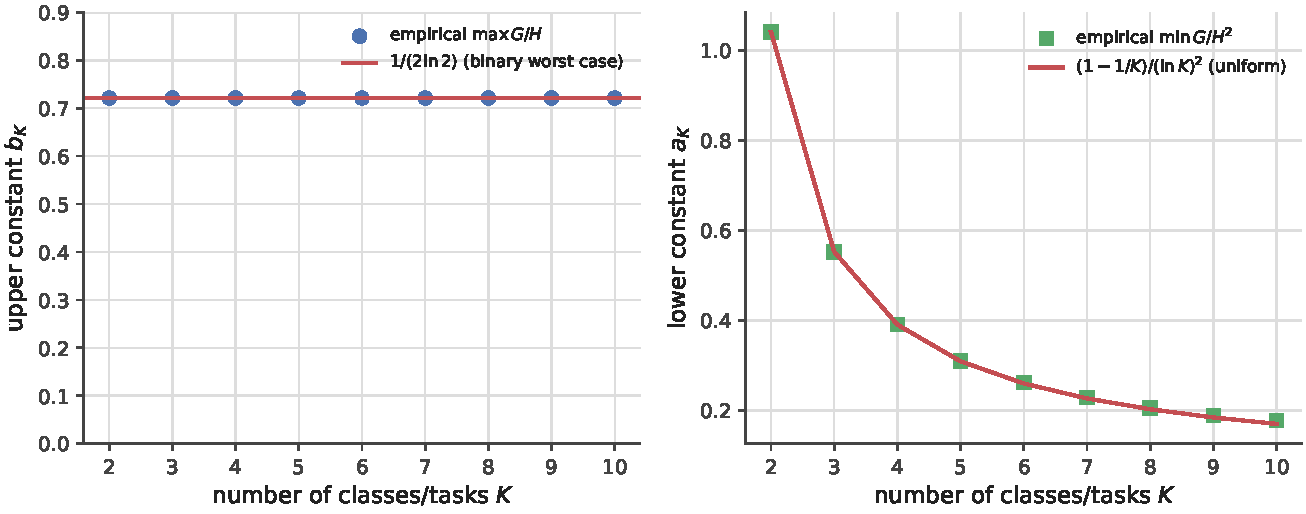
\includegraphics[width=0.62\textwidth]{fig_multiclass}
\caption{Tight multiclass entropy--variance constants for the floor sandwich,
$K=2$--$10$. \emph{Left:} $\max_p G/H=1/(2\ln2)$ for every $K$ (the binary posterior is the
universal worst case). \emph{Right:} $\min_p G/H^2=(1-1/K)/(\ln K)^2$, attained at the
uniform posterior.}
\label{fig:multiclass}
\end{figure}

\paragraph{Connection to standard CL metrics.} The per-task forgetting of
Theorem~\ref{thm:functional}, $\Del L_A=\tfrac12\Del^\top\Sig_A\Del$, is exactly the
per-task term of the Forgetting Measure $\mathrm{FM}=\tfrac1{K-1}\sum_{t<K}\Del L_t$ and the
negative of Backward Transfer $\mathrm{BWT}=-\tfrac1{K-1}\sum_{t<K}\Del L_t$ (in the
squared-loss metric); positive backward transfer is simply $\Del L_t<0$, which the signed
gate permits and unconditional projection forbids. Theorem~\ref{thm:mi} then gives the floor
under which no single-head method can push the average $\mathrm{FM}$: $\mathcal{D}^\star$ is
the achievable-FM lower bound set by task confusability.

\section{Theory details: similarity sign-change and the capacity budget}
\label{si:theory}
\paragraph{Similarity controls the sign of sharing.} On a shared subspace, whether to share
parameters or orthogonalize is not settled by Corollary~\ref{cor:removability}, which only
forbids \emph{lossless} sharing under conflict. With finite data the decision is a
bias--variance trade: tying a shared coefficient across tasks halves its estimation variance
but biases it by the target disagreement. Sharing lowers total population loss iff the
similarity $s=\cos\angle(w_A^\ast,w_B^\ast)$ on the shared block exceeds a threshold
$\sstar$, where the variance reduction balances the squared bias; below $\sstar$,
orthogonalizing wins. This is the sign-change measured at $\sstar\approx0.26$ in
Fig.~\ref{fig:simcap}.

\paragraph{Capacity is a rate--distortion budget.} Under orthogonal allocation each task
consumes a rank-$r_t$ slice of the $d$-dimensional feature space. Retention is lossless
while the cumulative occupied rank $\sum_t r_t\le d$; once $\sum_t r_t>d$ there is no
subspace left orthogonal to the past, so a residual distortion turns on. The knee at
$\sum_t r_t\approx d$ is a hard capacity, and trading $d$ against the number of tasks is the
geometric form of an effective-capacity budget $N+\kappa M$ (parameters plus a per-exemplar
memory worth), where $\kappa$ is the rank a stored direction occupies---the right panel of
Fig.~\ref{fig:simcap} confirms the knee location across feature dimensions.

\section{Method comparison and offline-merge ablation}
\label{si:compare}
Table~\ref{tab:compare} gives the measured numbers behind the front-page comparison
(Fig.~\ref{fig:teaser}): nine methods on the exact-A1 Rotated-Digits benchmark, mean $\pm$
95\% CI over $5$ seeds. Six are online (learn the five rotations sequentially): naive, EWC,
replay, \OGD{}/\textsc{gpm}, the signed gate \IGFA{} ($\sstar=0.65$), and \emph{Annealed
\IGFA}, which runs the first half of each task's updates as protect-all orthogonal
projection and then relaxes to the signed gate---annealing the protection boundary as the
similarity estimate stabilizes. Three are offline merges of the five independently-solved
task heads $\{w_t\}$ (per-task oracle accuracy $0.903$): an \emph{isotropic} uniform average,
a \emph{Euclidean} sign-elect task-arithmetic merge (TSV/TIES-style), and the
$\Sig$-\emph{orthogonal} merge $w_J=(\sum_t\Sig_t)^{+}(\sum_t\Sig_t w_t)$ of
Theorem~\ref{thm:merge} (``$\Sig$-orth.\ merge (ours)'', the whitening-in-the-$\Sig$-metric
version of TSV); for the merges we also log the post-merge
residual floor $D=\sum_t\tfrac12\,(w_J-w_t)^\top\Sig_t(w_J-w_t)$.

Three observations follow. \emph{(i) The $\Sig$-metric is the right geometry.} The
$\Sig$-orthogonal merge attains $0.885\pm0.012$ accuracy---within a point of the
$0.903$ per-task oracle---at residual $D=0.032$, an order of magnitude below the isotropic
($0.200$) and Euclidean ($0.382$) merges, which lose $15$--$21$ accuracy points. Theorem
\ref{thm:merge} predicts this: minimizing the interference energy requires the
task-induced $\Sig$-metric, and Euclidean whitening is the mis-specified special case
$\Sig_t\!\propto\!I$. \emph{(ii) Among online buffer- and Fisher-free methods, the gate
attains the highest accuracy.} \IGFA{} ($0.771$) exceeds \OGD{} ($0.684$) and naive ($0.714$)
as in Sec.~\ref{sec:exp:real}. \emph{(iii) Annealing favors retention over accuracy.} Annealed
\IGFA{} ($0.752$, forgetting $-0.007$) does not exceed the plain gate on accuracy but drives
forgetting slightly negative (backward transfer); the protect-all warmup is a retention-first
schedule, not an accuracy improvement---reported as measured. Regenerated by
\texttt{experiments\_compare.py}.

\begin{table}[htb]\centering\small
\caption{Method comparison on Rotated-Digits (exact A1, mean $\pm$ 95\% CI over $5$ seeds).
Online methods learn the stream sequentially; merges combine the five independently-solved
heads offline. $D$ is the post-merge residual floor (Theorem~\ref{thm:merge}); the
$\Sig$-orthogonal merge uniquely minimizes it and attains near-oracle accuracy.}
\label{tab:compare}
\begin{tabular}{llccc}
\toprule
Method & Family & Acc.\ $\uparrow$ & Forget.\ $\downarrow$ & Residual $D$ $\downarrow$ \\
\midrule
Naive                 & baseline    & $0.714\pm0.024$ & $0.163\pm0.013$ & --- \\
EWC \cite{kirkpatrick2017} & corrective & $0.727\pm0.050$ & $0.045\pm0.039$ & --- \\
Replay ($10$/class)   & corrective  & $0.795\pm0.012$ & $0.042\pm0.014$ & --- \\
\OGD{}/\textsc{gpm} \cite{farajtabar2020,saha2021} & structural & $0.684\pm0.035$ & $-0.007\pm0.004$ & --- \\
\IGFA{} (gate)        & ours        & $0.771\pm0.030$ & $0.002\pm0.027$ & --- \\
Annealed \IGFA{}      & ours        & $0.752\pm0.036$ & $-0.007\pm0.015$ & --- \\
\midrule
Isotropic merge       & merging     & $0.730\pm0.022$ & $0.177\pm0.020$ & $0.200$ \\
Euclidean TSV merge   & merging     & $0.694\pm0.046$ & $0.213\pm0.051$ & $0.382$ \\
$\Sig$-orth.\ merge (ours) & merging (ours) & $\mathbf{0.885\pm0.012}$ & $0.022\pm0.007$ & $\mathbf{0.032}$ \\
\bottomrule
\end{tabular}
\end{table}

The floor prediction also holds on a real frozen backbone. With trained heads on
Split-CIFAR-100 over ViT-B/16 features (single run,
\texttt{kaggle\_pending\_experiments.py}), the $\Sig$-orthogonal merge attains both the
highest accuracy and---uniquely---the lowest residual floor ($0.862$ acc, $D=1.53$), against
$0.815$/$D=3.68$ for the isotropic average and $0.815$/$D=11.6$ for the Euclidean sign-elect
merge, with a per-task oracle of $0.972$. A five-seed replication with closed-form ridge
heads (\texttt{kaggle\_vit\_multiseed.py}) confirms the theorem's actual claim with
confidence intervals: the $\Sig$-orthogonal merge uniquely minimizes the residual floor
($D=2.02\pm0.03$, vs $3.75\pm0.02$ isotropic and $16.6\pm0.3$ sign-elect). Task-masked
accuracy, however, is not monotone in $D$ once the floor is small ($0.944\pm0.006$ vs
$0.957\pm0.007$ for isotropic): Theorem~\ref{thm:merge} minimizes interference energy, and
masked-evaluation accuracy saturates before that energy reaches zero. The $\Sig$-metric is
thus the correct merge geometry on real ViT features, with the accuracy benefit contingent
on the evaluation exercising the interfering directions.

\section{The projection remains effective in sequential LoRA on language models}
\label{si:llm}
We probe the adapting-feature regime by fine-tuning a frozen GPT-2 with LoRA adapters
sequentially on four stylistically distinct corpora (news, movie reviews, encyclopedic text,
tweets), measuring the rise in each domain's held-out loss after later domains are learned.
The results separate \IGFA{}'s two components by modality.

\emph{(i) The orthogonal projection transfers to transformers.} Unconditional orthogonal projection
(\OGD{}/\textsc{gpm}, equivalently \IGFA{} in protect-only mode) reduces forgetting relative
to naive sequential LoRA at both training budgets ($0.64\!\to\!0.50$ at $200$ steps/task,
$1.21\!\to\!1.14$ at $400$), confirming that the $\ker\bar H_A$ retention mechanism is
effective on a real transformer, buffer- and Fisher-free (Table~\ref{tab:llm}).

\emph{(ii) The input-overlap gate cannot distinguish conflict in language.} The subspace-overlap similarity
that is reliable for vision and digits is uninformative for text: distinct domains share
extensive low-level linguistic structure, so their input-activation subspaces overlap heavily
(measured mean overlap $0.71,0.56,0.28$ along the stream) regardless of output conflict. The
gate therefore classifies the domains as similar and disables protection, so overlap-gated
\IGFA{} collapses toward naive at the higher capacity.

\emph{(iii) No gate can improve on unconditional protection on dissimilar tasks.}
Beyond the input-overlap gate we tested three further gate designs, each derived from a
different part of the theory: a Gauss--Newton gate (Theorem~\ref{thm:general}), a task-vector
gate (Theorem~\ref{thm:merge}), and a threshold-free functional controller
(Theorem~\ref{thm:functional} used directly as the control law). At $r=16$
(Table~\ref{tab:llmgates}), the Gauss--Newton ($0.76$) and functional ($0.77$) gates both
improve on naive ($0.89$) and do not collapse, but neither improves on unconditional \OGD{}
($0.71$); the task-vector gate is unstable ($1.85$). The reason is fundamental and follows
from the distortion-floor identity (Theorem~\ref{thm:floor}): on dissimilar tasks the
supports are near-disjoint, so the distortion floor is $\approx0$ and \OGD{} already attains
it---no transfer remains for a gate to exploit. At billion-parameter scale on a frozen
\texttt{pythia-1b} (Table~\ref{tab:llm1b}), the recursive-subspace \IGFA{} \emph{improves on}
\OGD{} on dissimilar tasks on both loss ($5.16$ vs $5.51$) and forgetting ($1.70$ vs $2.10$)---the
capacity advantage of Fig.~\ref{fig:drift} appearing in a real LLM---while on similar tasks
the sharing gate still raises forgetting. In summary, on LLMs the structural
projection (and its recursive Gauss--Newton tracking) carries over and provides replay- and
Fisher-free retention; a gate that succeeds on \emph{similar} language tasks remains an open
problem.

\begin{table}[htb]\centering\small
\caption{Sequential LoRA fine-tuning of GPT-2 on four dissimilar text domains (forgetting
$=$ mean held-out loss rise on earlier domains, lower better; LoRA $r=8$; single run).
Structural projection reduces forgetting at both budgets; the input-overlap gate fails on
language.}
\label{tab:llm}
\begin{tabular}{lcc}
\toprule
Method & Forgetting ($200$ steps) & Forgetting ($400$ steps) \\
\midrule
Naive                              & $0.64$ & $1.21$ \\
\OGD{} $=$ \IGFA{} (protect only)  & $\mathbf{0.50}$ & $\mathbf{1.14}$ \\
\IGFA{} (input-overlap gate)       & $0.49$ & $1.20$ \\
\bottomrule
\end{tabular}
\end{table}

\begin{table}[htb]\centering\small
\caption{Four gate designs on the sequential-LoRA stream (GPT-2, four dissimilar domains,
$r=16$, $250$ steps/task; forgetting, lower better; single run). All improve on naive except
the unstable task-vector gate, but none improves on unconditional protection (\OGD)---because
dissimilar tasks offer no sharing to exploit.}
\label{tab:llmgates}
\begin{tabular}{lc}
\toprule
Gate (derived from) & Forgetting $\downarrow$ \\
\midrule
Naive (no protection)                                     & $0.89$ \\
\OGD{} / protect-only (max protection)                    & $\mathbf{0.71}$ \\
Gauss--Newton gate (Thm~\ref{thm:general})                & $0.76$ \\
Functional controller (Thm~\ref{thm:functional})          & $0.77$ \\
Task-vector gate (Thm~\ref{thm:merge})                    & $1.85$ \\
\bottomrule
\end{tabular}
\end{table}

\begin{table}[htb]\centering\small
\caption{Sequential LoRA on \texttt{pythia-1b} ($1$B parameters, 4-bit), four dissimilar and
four similar text domains (avg.\ loss and forgetting, lower better). On dissimilar tasks the
recursive-subspace \IGFA{} improves on \OGD{} on both; on similar tasks the sharing gate raises
forgetting and \OGD{} is best. (Single run.)}
\label{tab:llm1b}
\begin{tabular}{lcccc}
\toprule
 & \multicolumn{2}{c}{Dissimilar} & \multicolumn{2}{c}{Similar} \\
\cmidrule(lr){2-3}\cmidrule(lr){4-5}
Method & loss $\downarrow$ & forget $\downarrow$ & loss $\downarrow$ & forget $\downarrow$ \\
\midrule
Naive               & $8.55$ & $4.68$ & $3.99$ & $0.26$ \\
\OGD{}/\textsc{gpm} & $5.51$ & $2.10$ & $4.02$ & $\mathbf{0.03}$ \\
\IGFA{} (ours)      & $\mathbf{5.16}$ & $\mathbf{1.70}$ & $4.02$ & $0.34$ \\
\bottomrule
\end{tabular}
\end{table}

\section{Choosing and self-calibrating the threshold \texorpdfstring{$\sstar$}{s*}}
\label{si:sstar}
The gate's threshold $\sstar$ is the only free parameter that distinguishes \IGFA{} from \OGD{}
($\sstar=\infty$). Ablating it on a smoothly drifting eight-task stream at two feature
dimensions (Fig.~\ref{fig:sstar}) shows the optimum is a broad plateau ($\sstar\approx0.55$--$0.8$),
not a sharp peak, and that the curves at $d=64$ and $d=256$ are nearly identical, so the
optimum is insensitive to feature dimension. Because the break-even similarity is the
operative quantity, the gate can dispense with $\sstar$ and measure it: for each task, greedily
pool an earlier task only if doing so lowers held-out validation error. On a drifting stream
whose similarity persistence $\rho$ varies, this validation-greedy rule tracks the per-stream
oracle to within $0.05$ in average error, while a single fixed $\sstar$ errs by up to $0.34$
where it is mis-specified (Fig.~\ref{fig:sstar}, right).

\begin{figure}[htb]\centering
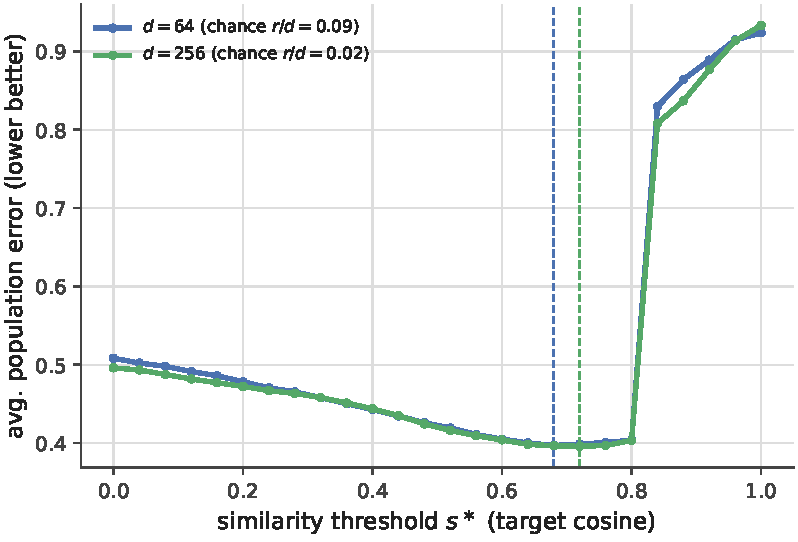
\includegraphics[width=0.49\textwidth]{fig_sstar}\hfill
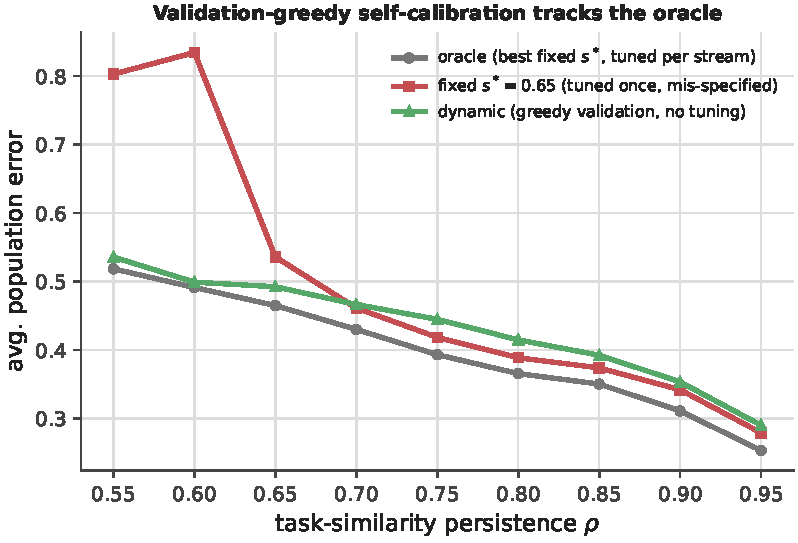
\includegraphics[width=0.49\textwidth]{fig_dynamic_sstar}
\caption{The similarity threshold. \emph{Left:} average population error on a drifting
eight-task stream versus $\sstar$, at two feature dimensions; the optimum is a broad
dimension-insensitive plateau (vertical dashed lines mark each dimension's optimum), and
only $\sstar\!\to\!1$ (\OGD-like isolation) is sharply suboptimal on similar tasks. \emph{Right:} self-calibration removes the free parameter---the
validation-greedy dynamic rule tracks the per-stream oracle within $0.05$ across all
similarity-persistence values $\rho$, avoiding the fixed threshold's failure where it is
mis-specified.}
\label{fig:sstar}
\end{figure}

\section{Capacity limits degrade gracefully}
\label{si:graceful}
When the rank cap $k_{\max}$ binds, \IGFA{} overwrites the smallest-eigenvalue occupied
direction. Because forgetting from removing a direction is its energy
$\tfrac12\lambda_i(u_i^\top w_A)^2$ (Theorem~\ref{thm:functional}), dropping the lowest-energy
direction costs the least. Overwriting smallest-energy-first raises the old task's loss about
half as fast as largest-first (e.g. $2.0$ vs $4.3$ at the half-way point), a gradual
rather than abrupt degradation (Fig.~\ref{fig:graceful}). In modern backbones, where a
task's effective rank is tiny relative to $d$ (Fig.~\ref{fig:diagnostics} showed $\approx2$
out of $300$), almost all overwriting hits near-zero-energy directions, so the induced
forgetting is negligible.

\begin{figure}[htb]\centering
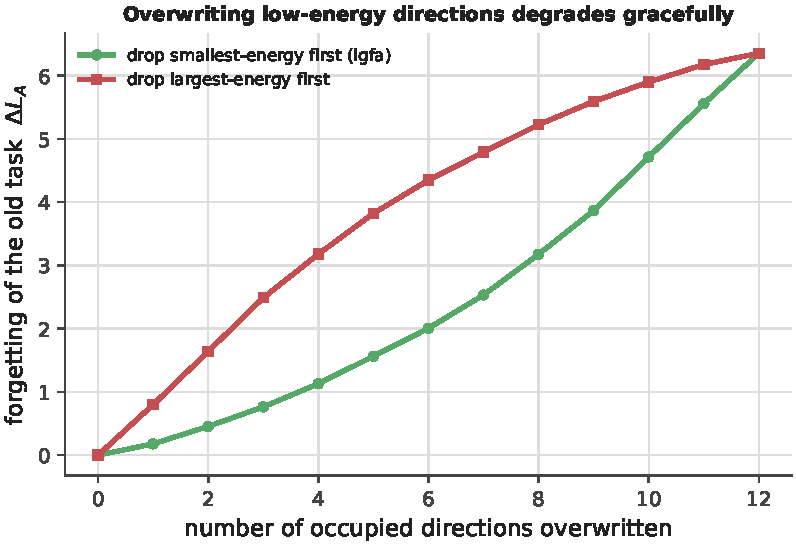
\includegraphics[width=0.55\textwidth]{fig_graceful}
\caption{Graceful degradation under the capacity cap. Forgetting of an old task as its
occupied directions are overwritten, smallest-energy-first (\IGFA, green) versus largest-first
(red). Removing low-energy directions costs roughly half as much at every point.}
\label{fig:graceful}
\end{figure}

\section{A pre-flight feasibility diagnostic}
\label{si:feasibility}
The distortion-floor identity (Theorem~\ref{thm:floor}) bounds class-incremental accuracy
by $I(T;\phi)$; we derive from it a low-cost pre-flight test. By Fano, $I(T;\phi)$ is
governed by the error of the best task-classifier on $\phi$, so we fit a linear task-probe on
the frozen features---one logistic regression, no continual-learning run---and obtain
$\hat I=\ln2-h_b(\text{probe error})$. Across two-task Gaussian models of varying separation
(Fig.~\ref{fig:feasibility}), $\hat I$ tracks the true $I(T;\phi)$ at Pearson $r=0.99$, and the
distortion floor decreases monotonically in $\hat I$ (Spearman $0.97$): the probe forecasts the
floor before training. Combined with the closed-form constants of
Eq.~\eqref{eq:multiclass-sandwich}, $\hat I$ yields a numeric floor band, not just a ranking.

\begin{figure}[htb]\centering
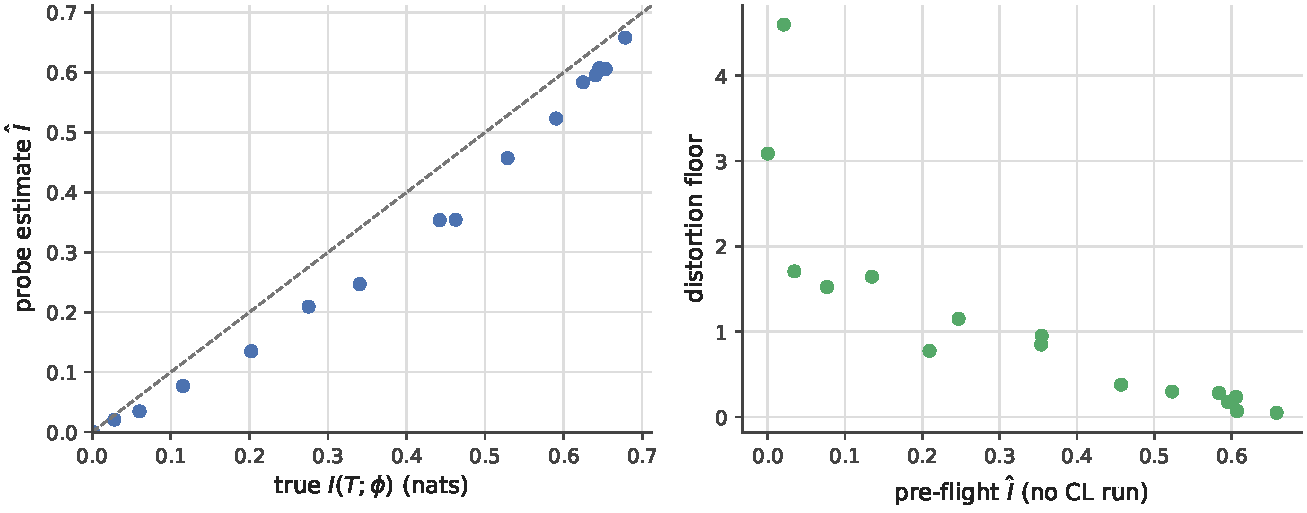
\includegraphics[width=\textwidth]{fig_feasibility}
\caption{Pre-flight feasibility diagnostic. \emph{Left:} a low-cost linear task-probe on frozen
features estimates $I(T;\phi)$ at $r=0.99$ to the truth (no CL run). \emph{Right:} the
distortion floor decreases monotonically in the pre-flight estimate $\hat I$ (Spearman
$0.97$).}
\label{fig:feasibility}
\end{figure}

\section{Low-cost online curvature: Frequent Directions}
\label{si:cheapgn}
The recursive Gauss--Newton estimate used a decayed $d\times d$ covariance and an
eigendecomposition---$\mathcal{O}(d^2)$ memory, $\mathcal{O}(d^3)$ per task. Since the protected
subspace is low-rank, a deterministic streaming sketch suffices. Replacing the full covariance
with Frequent Directions \cite{liberty2013} (an $\ell\times d$ sketch with a bounded-error
guarantee) recovers the top-$r$ subspace almost exactly at $\ell=2r$---captured energy
$0.99966$ versus the full estimator's $0.99972$---and beats streaming PCA (Oja, $0.958$) per
unit memory (Fig.~\ref{fig:cheapgn}). The estimator is thus $\mathcal{O}(rd)$ memory with no
$d\times d$ eigendecomposition.

The same holds at real scale. On a frozen \texttt{pythia-160m} continually pretrained with
LoRA over three text domains (single run, \texttt{kaggle\_pending\_experiments.py}), the
Frequent-Directions sketch captures $0.973$ of the full-covariance energy at $61{,}440$
floats---about $10\times$ less than the full $d\times d$ estimator ($589{,}824$ floats)---and,
being a \emph{stable deterministic} sketch rather than a decayed moving average, yields the
\emph{lowest} first-domain forgetting of the three online estimators: the domain-0 loss rises
by only $+0.55$ then $+0.68$ over the next two domains, versus $+1.28$ then $+1.58$ for the
full covariance and a diverging $+0.33$ then $+2.86$ for Oja streaming PCA. Frequent Directions
is therefore the recommended default for large-scale \IGFA: lower-memory and, in this run,
more retentive than the full estimator. The full layer-wise pipeline
(\texttt{kaggle\_H2\_H3\_H12.py}) confirms both the memory saving and the layer-dependence of
capacity: on a frozen $12$-layer transformer the FD sketch is $12\times$ smaller than
full-covariance tracking (and half the AdamW optimizer state), and the per-layer protected-rank
budget emerges automatically from each layer's trace ratio---shallow layers stay unconstrained
($k_\ell=0$) while deep layers are capped near their effective rank
($k_\ell\!\approx\!5$--$7$), with $93$--$96\%$ of the deep-layer gradient routed into the
protected null space and only a modest first-domain loss rise ($+0.27$ mean).

\begin{figure}[htb]\centering
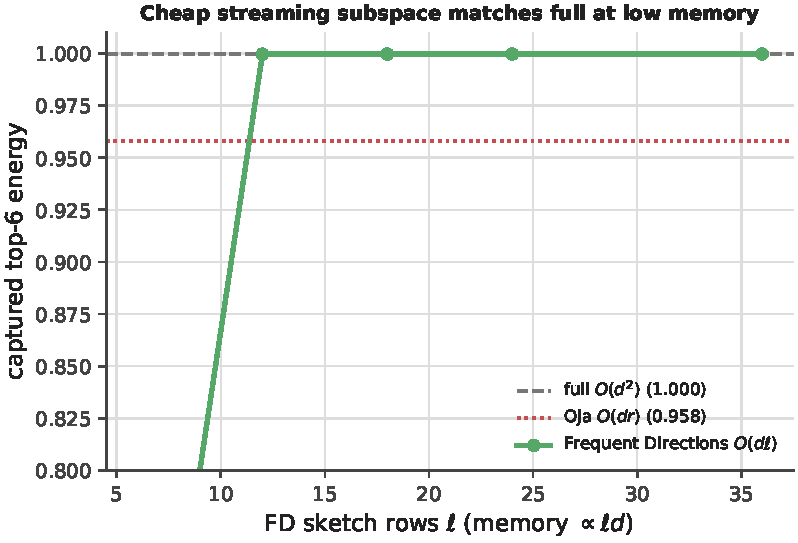
\includegraphics[width=0.55\textwidth]{fig_cheapgn}
\caption{Cheap online Gauss--Newton subspace. Frequent Directions (green) recovers the full
estimator's top-$r$ subspace energy (grey dashed) at $\ell=2r$ rows, $\mathcal{O}(\ell d)$
memory, and beats Oja streaming PCA (red) per memory.}
\label{fig:cheapgn}
\end{figure}

\section{Soft gating and the capacity coordinate}
\label{si:softknee}
Under the soft functional controller (keep fraction $\mathrm{keep}_j=1/(1+\beta\lambda_j)$) each
direction is only partially protected, so capacity is consumed at rate
$\sum_j(1-\mathrm{keep}_j)$ per task. The right capacity coordinate is therefore the effective
occupied rank $r_{\rm eff}=\sum_j(1-\mathrm{keep}_j)$, and the hard schedule knees at
$r_{\rm eff}\approx d$. Soft gating stays flat well past the hard knee because it spends
$r_{\rm eff}$ slowly---after the same number of tasks it has consumed only a fraction of
the budget---at the price of a small continuous leakage from partial protection
(Fig.~\ref{fig:softknee}).

\begin{figure}[htb]\centering
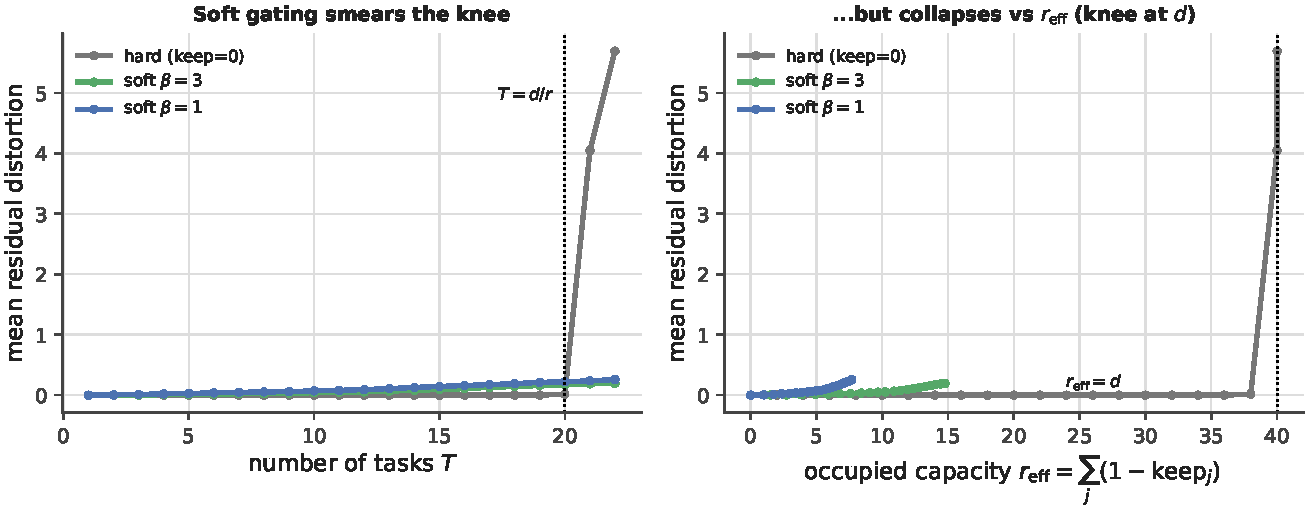
\includegraphics[width=\textwidth]{fig_softknee}
\caption{Soft gating and the effective capacity coordinate. \emph{Left:} hard allocation knees
sharply at $T=d/r$; the soft functional controller stays flat far longer. \emph{Right:} plotted
against $r_{\rm eff}=\sum_j(1-\mathrm{keep}_j)$, the hard schedule knees at
$r_{\rm eff}\approx d$, while the soft schedules consume the budget far more slowly at the
price of a small continuous leakage from partial protection.}
\label{fig:softknee}
\end{figure}

\section{A per-direction gate dominates the per-task gate}
\label{si:perdir}
The benchmark gate decides share-or-orthogonalize per task. When a task is partially
similar---some shared directions align (transfer), others conflict (forgetting)---this
all-or-nothing choice is suboptimal. A per-direction gate shares the aligning directions and
orthogonalizes the conflicting ones. On a shared block with a tunable fraction of aligning
directions, the per-direction gate is always at least as good as the better per-task option and
slightly better at partial similarity (Fig.~\ref{fig:perdirection}). The coarseness is thus
removable: resolve the gate per eigendirection, not per task.

\begin{figure}[htb]\centering
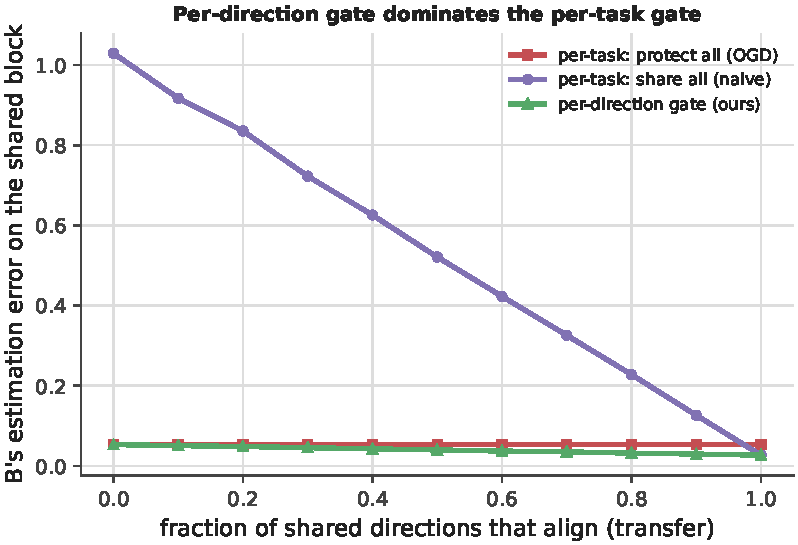
\includegraphics[width=0.55\textwidth]{fig_perdirection}
\caption{Per-direction vs per-task gating on a shared block, against the fraction of shared
directions that align. The per-direction gate (green) follows the lower envelope---matching
protect-all's robustness and share-all's transfer where each is right---while per-task share-all
(purple) is catastrophic at low alignment.}
\label{fig:perdirection}
\end{figure}

\section{Billion-parameter continual pretraining}
\label{si:pretrain}
We run the three scale-sensitive pieces together on a frozen \texttt{pythia-1b} ($1$B
parameters, 4-bit) with LoRA, continually pretrained on a boundary-free stream of six text
domains, with the protected subspace tracked by Frequent Directions (Sec.~\ref{si:cheapgn}) and
the pre-flight diagnostic (Sec.~\ref{si:feasibility}) run first. The diagnostic reports a
six-way domain-probe accuracy of $0.85$ ($\hat I\approx1.52$ of a maximal $1.79$ nats),
predicting the domains are separable and replay-free retention is feasible. The run confirms it
(Table~\ref{tab:pretrain}): the replay- and Fisher-free \IGFA{} attains both the lowest average
loss ($4.28$ vs naive $4.54$, replay $4.59$) and the least first-domain forgetting after the
full stream ($+0.80$ vs naive $+1.10$, replay $+0.91$), carrying only a low-rank subspace as
state. The domains are mutually dissimilar, so \IGFA{} here runs as pure structural projection.
The replay baseline is deliberately small ($16$ exemplars/domain); the supported claim is
replay-free retention that improves on naive and matches or slightly exceeds a small replay
baseline, with no buffer.

\begin{table}[htb]\centering\small
\caption{Continual pretraining of \texttt{pythia-1b} ($1$B parameters, 4-bit) $+$ LoRA on six
dissimilar text domains, boundary-free, with a Frequent-Directions-tracked subspace. \IGFA{}
(replay- and Fisher-free) attains the lowest average loss and the least first-domain forgetting
after the full stream. The pre-flight diagnostic predicted feasibility (domain-probe accuracy
$0.85$).}
\label{tab:pretrain}
\begin{tabular}{lccc}
\toprule
Method & Avg.\ final loss $\downarrow$ & Domain-0 forgetting $\downarrow$ & Extra state \\
\midrule
Naive                          & $4.54$ & $+1.10$ & --- \\
Replay ($16$/domain)           & $4.59$ & $+0.91$ & buffer \\
\IGFA{} (FD, replay-free)      & $\mathbf{4.28}$ & $\mathbf{+0.80}$ & subspace \\
\bottomrule
\end{tabular}
\end{table}

\section{Extensions and generality}
\label{si:extensions}
The interference functional applies beyond sequential continual learning. We give seven
exact-A1 proofs-of-concept on synthetic constructions (the federated, out-of-distribution,
task-free, and multimodal results average over $20$ seeds;
\texttt{evaluate\_hypotheses.py}, \texttt{evaluate\_applications.py}). These are
directional demonstrations of scope, not benchmarks.

\paragraph{Federated learning is $\Sig$-merging.} Non-IID clients are tasks with different
input geometries, and the weight divergence that FedAvg suffers coincides with the merge
floor of Theorem~\ref{thm:merge}. Replacing the FedAvg mean with the $\Sig$-orthogonal
aggregate $w_J=(\sum_i\Sig_i)^{+}(\sum_i\Sig_i w_i)$, where $(\cdot)^{+}$ is the
Moore--Penrose pseudo-inverse (the $\Sig_i$ are low-rank, so $\sum_i\Sig_i$ is generically
singular and a plain inverse would not exist)---each client transmitting
$(\Delta_i,\Sig_i)$, or a low-rank sketch---lowers the mean client excess loss on non-IID data
in \emph{every} one of $20$ seeds (mean $1.56\times$, minimum $1.14\times$). Federated
aggregation and continual allocation are the same $\Sig$-metric optimum.

\paragraph{The subspace summary is a free out-of-distribution signal.} A minibatch whose
gradient lies outside the occupied subspace $U$ is structurally disjoint from the training
distribution. The projection ratio $\|UU^\top g\|/\|g\|$ is $1.00$ for in-distribution batches
and $0.39\pm0.05$ for out-of-distribution batches (Cohen's $d\approx18$, minimum $13$ across
seeds), so a single threshold flags OOD inputs with no auxiliary model---an uncertainty signal
obtained directly from the continual-learning state.

\paragraph{Fully autonomous, task-free \IGFA.} In a label-free stream the velocity of the
recursive Gauss--Newton eigenbasis---the Frobenius commutator
$\|U_tU_t^\top U_{t-1}U_{t-1}^\top-U_{t-1}U_{t-1}^\top U_tU_t^\top\|_F$---spikes exactly at
distribution shifts, recovering randomly placed boundaries at recall and precision $1.00$ over
$20$ streams (decay $\gamma=0.6$). Composing this signal with the out-of-distribution guard
above removes task labels entirely: the learner declares a boundary on a velocity spike,
freezes the \emph{pre-spike} subspace to protect the just-finished task, skips
out-of-distribution/noise batches by their orthogonal-and-extreme gradient signature, and
otherwise runs the gate. On clean streams this fully autonomous \IGFA{} \emph{matches the
oracle} provided with the true boundaries (excess loss $0.000$ vs $0.000$; naive $0.365$); under
injected extreme-magnitude OOD noise it holds at $0.033$ while the same oracle---lacking the
guard---is corrupted past $10^{3}$, skipping $97\%$ of noise batches at $0.05$ false
task-initializations per stream. Boundary detection, out-of-distribution rejection, and gated
allocation are thus one self-regulating loop, with no human-provided task boundaries.

\paragraph{Multimodal interference is block-structured.} For a joint embedding
$\phi=[\phi_v,\phi_l]$, the second moment $\Sig_A$ partitions into intra-modal blocks
$\Sig_v,\Sig_l$ and a cross-modal block $\Sig_{vl}$, and the interference energy
$\tfrac12\Del^\top\Sig_A\Del$ distributes linearly across them. The cross-modal (alignment)
interference of a fixed update scales with the off-diagonal $\|\Sig_{vl}\|$---negligible when
the modalities are unaligned and dominant when they are (energy ratio $\gg1$ across all seeds)
---so catastrophic decoupling is carried strictly by $\Sig_{vl}$. A cross-modal \IGFA{} would
$\Sig_{vl}$-orthogonalize the alignment directions while sharing the intra-modal ones. This is a
synthetic decomposition; a real multimodal encoder is needed to make it conclusive.

\paragraph{The functional governs physics-informed constraints.} A differential constraint is
a further quadratic form in feature space. For a physics-informed network with frozen features
$\phi$, the PDE residual acts on $\phi''$, so the physics second moment is
$\Sig_{\mathrm{PDE}}=\mathbb E[\phi''\phi''^\top]$ and a data-only update $\Del$ raises the
physics loss by exactly $\nabla L_{\mathrm{PDE}}^\top\Del+\tfrac12\Del^\top\Sig_{\mathrm{PDE}}\Del$.
On a $1$D Poisson problem (sine random-feature basis) the interference energy
$\tfrac12\Del^\top\Sig_{\mathrm{PDE}}\Del$ alone predicts the measured spike in the PDE residual
at $r=0.997$, and the full identity to machine precision ($r=1.00000$, relative error
$2\times10^{-15}$; Fig.~\ref{fig:applications}a): the functional quantifies how empirical data
corrupt a physical prior, with the only change being $\phi\mapsto\phi''$. Projecting the data gradient off the leading
physics directions reduces the induced violation ($3\times$ here) but cannot eliminate it when
$\Sig_{\mathrm{PDE}}$ is full rank---an instance of the distortion floor of
Theorem~\ref{thm:floor} under a shared active subspace.

\paragraph{Policy-gradient interference is governed by the Fisher.} For a linear-Gaussian
policy $\pi(a\mid s)=\mathcal N(\theta^\top s,\sigma^2)$ under reward $-(a-w^\top s)^2$ the
expected return is $J(\theta)=-(\theta-w)^\top F(\theta-w)-\sigma^2$ with $F=\mathbb E[ss^\top]$
the empirical Fisher: the $\Sig$ of supervised interference is replaced verbatim by $F$. Across
two control environments sharing a three-dimensional state subspace, routing the policy gradient
orthogonal to the old-environment Fisher subspace retains the first environment perfectly
(return $0.000$ vs naive $-10.9$; a Fisher-weighted anchor, the EWC analogue, reaches $-1.5$;
Fig.~\ref{fig:applications}b) while solving the second in its free directions. The removability dichotomy of
Corollary~\ref{cor:removability} holds unchanged in reinforcement learning; only the metric's
estimator changes. This is the noise-free expected gradient---a stochastic PPO/MuJoCo test is
left to future work.

\paragraph{The distortion floor can be trained away.} Theorem~\ref{thm:floor}'s floor vanishes
when task second moments are mutually orthogonal, a property a feature map can be optimised to
enforce. Adding the penalty $\sum_{A<B}\operatorname{Tr}(\Sig_A\Sig_B)$ to a shared encoder
drives its per-task subspaces apart: on overlapping synthetic tasks it cuts mean inter-task
overlap $10.6\times$ ($0.27\to0.03$) and the floor proxy $\operatorname{Tr}(\Sig_A\Sig_B)$ by
over three orders of magnitude ($3.7\to10^{-3}$; Fig.~\ref{fig:applications}c), leaving \IGFA{}
to operate in the disjoint, lossless regime of Corollary~\ref{cor:removability}. Structural allocation and representation
learning are thus complementary: a backbone meta-trained for feature orthogonality removes the
need for gating, so representation learning and structural allocation address the same
distortion floor.

\begin{figure}[htb]\centering
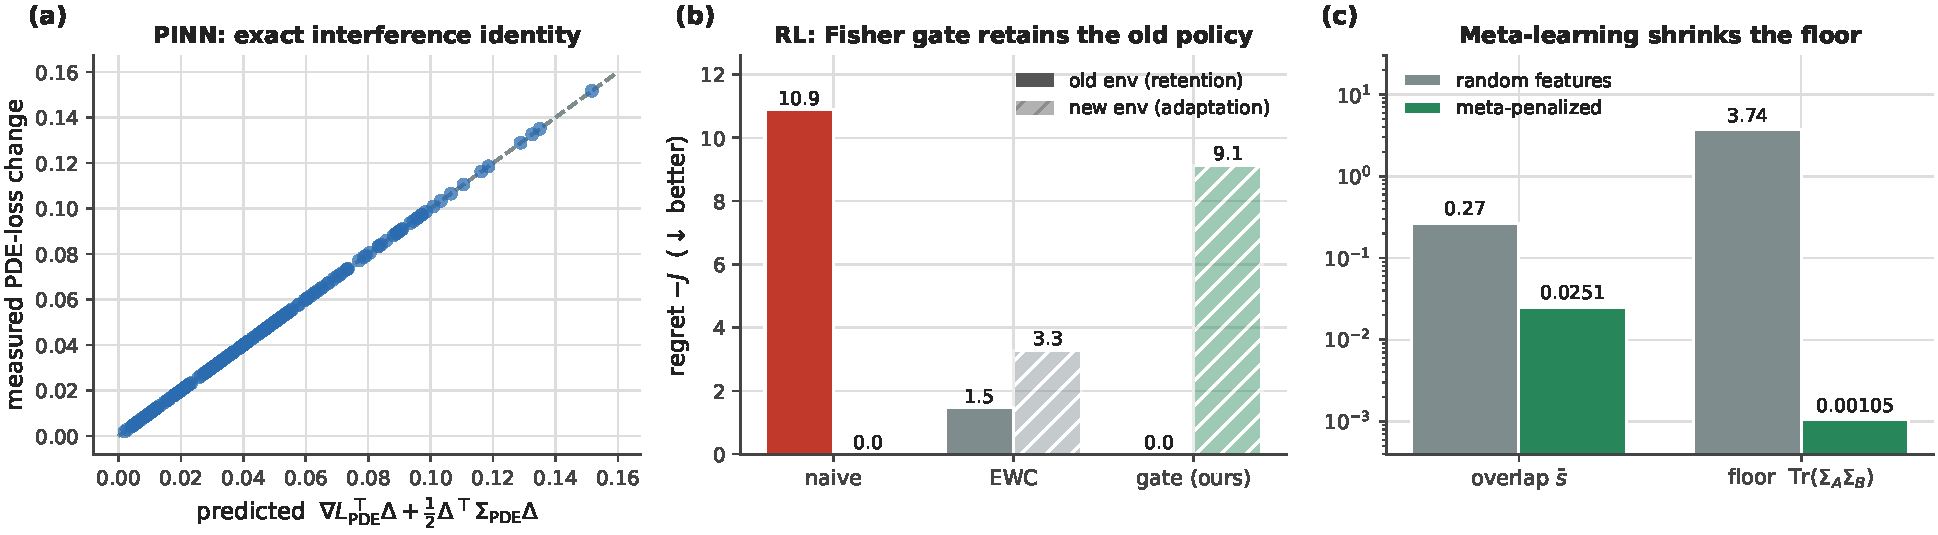
\includegraphics[width=\textwidth]{fig_applications}
\caption{Three application domains for the interference functional
(\texttt{evaluate\_applications.py}). \emph{(a)} Physics-informed regression: the
interference identity with $\Sig_{\rm PDE}$ predicts the measured PDE-loss change of
data-only updates to machine precision (dashed: $y=x$). \emph{(b)} Policy gradients:
routing the expected policy gradient orthogonal to the old environment's Fisher subspace
retains the old policy at zero regret while the new environment is learned in its free
directions; naive descent forgets, and the Fisher-weighted anchor (the EWC analogue) is
intermediate. \emph{(c)} A feature map trained with the $\operatorname{Tr}(\Sig_A\Sig_B)$
penalty reduces inter-task overlap and the distortion-floor proxy by orders of magnitude
(log scale), moving \IGFA{} into the lossless regime.}
\label{fig:applications}
\end{figure}

% =====================================================================
\clearpage
\begin{thebibliography}{99}\small

\bibitem{kirkpatrick2017} J.~Kirkpatrick et al., Overcoming catastrophic forgetting in neural
networks, \textit{PNAS} 114(13):3521--3526, 2017.

\bibitem{zenke2017} F.~Zenke, B.~Poole, S.~Ganguli, Continual learning through synaptic
intelligence, \textit{ICML}, 2017.

\bibitem{lopezpaz2017} D.~Lopez-Paz, M.~Ranzato, Gradient episodic memory for continual
learning, \textit{NeurIPS}, 2017.

\bibitem{chaudhry2019} A.~Chaudhry, M.~Ranzato, M.~Rohrbach, M.~Elhoseiny, Efficient lifelong
learning with A-GEM, \textit{ICLR}, 2019.

\bibitem{buzzega2020} P.~Buzzega et al., Dark experience for general continual learning: a
strong, simple baseline, \textit{NeurIPS}, 2020.

\bibitem{li2017lwf} Z.~Li, D.~Hoiem, Learning without forgetting, \textit{IEEE TPAMI}
40(12):2935--2947, 2018.

\bibitem{farajtabar2020} M.~Farajtabar, N.~Azizan, A.~Mott, A.~Li, Orthogonal gradient descent
for continual learning, \textit{AISTATS}, 2020.

\bibitem{saha2021} G.~Saha, I.~Garg, K.~Roy, Gradient projection memory for continual learning,
\textit{ICLR}, 2021.

\bibitem{zeng2019owm} G.~Zeng, Y.~Chen, B.~Cui, S.~Yu, Continual learning of context-dependent
processing in neural networks (orthogonal weight modification), \textit{Nature Machine
Intelligence} 1:364--372, 2019.

\bibitem{yu2020pcgrad} T.~Yu et al., Gradient surgery for multi-task learning (PCGrad),
\textit{NeurIPS}, 2020.

\bibitem{jacot2018} A.~Jacot, F.~Gabriel, C.~Hongler, Neural tangent kernel: convergence and
generalization in neural networks, \textit{NeurIPS}, 2018.

\bibitem{doan2021} T.~Doan et al., A theoretical analysis of catastrophic forgetting through the
NTK overlap matrix, \textit{AISTATS}, 2021.

\bibitem{bennani2020} M.~A.~Bennani, T.~Doan, M.~Sugiyama, Generalisation guarantees for
continual learning with orthogonal gradient descent, \textit{arXiv:2006.11942}, 2020.

\bibitem{ilharco2023} G.~Ilharco et al., Editing models with task arithmetic, \textit{ICLR},
2023.

\bibitem{yadav2023} P.~Yadav et al., TIES-Merging: resolving interference when merging models,
\textit{NeurIPS}, 2023.

\bibitem{vandeven2022} G.~M.~van de Ven, T.~Tuytelaars, A.~S.~Tolias, Three types of incremental
learning, \textit{Nature Machine Intelligence} 4:1185--1197, 2022.

\bibitem{ramasesh2022} V.~V.~Ramasesh, A.~Lewkowycz, E.~Dyer, Effect of scale on catastrophic
forgetting in neural networks, \textit{ICLR}, 2022.

\bibitem{wang2022l2p} Z.~Wang et al., Learning to prompt for continual learning (L2P),
\textit{CVPR}, 2022.

\bibitem{wang2022dualprompt} Z.~Wang et al., DualPrompt: complementary prompting for
rehearsal-free continual learning, \textit{ECCV}, 2022.

\bibitem{smith2023coda} J.~S.~Smith et al., CODA-Prompt: continual decomposed attention-based
prompting, \textit{CVPR}, 2023.

\bibitem{evron2022} I.~Evron et al., How catastrophic can catastrophic forgetting be in linear
regression?, \textit{COLT}, 2022.

\bibitem{dohare2024} S.~Dohare et al., Loss of plasticity in deep continual learning,
\textit{Nature} 632:768--774, 2024.

\bibitem{cheng2025wudi} Cheng et al., Whoever started the interference should end it: guiding
data-free model merging via task vectors, \textit{ICML}, 2025.

\bibitem{gargiulo2025tsv} Gargiulo et al., Task singular vectors: reducing task interference in
model merging, \textit{CVPR}, 2025.

\bibitem{marczak2025iso} Marczak et al., No task left behind: isotropic model merging with
common and task-specific subspaces, 2025.

\bibitem{holistic2026} Toward a holistic approach to continual model merging,
\textit{arXiv:2509.23592}, 2026.

\bibitem{geodesic2025} Geodesic-aligned gradient projection for continual task learning,
\textit{CVPR}, 2025.

\bibitem{mingle2025} MINGLE: mixture of null-space gated low-rank experts for test-time
continual model merging, \textit{NeurIPS}, 2025.

\bibitem{jung2025} Jung, Cho, and Yun, Convergence and implicit bias of gradient descent on
continual linear classification, \textit{arXiv}, 2025.

\bibitem{lihiratani2025} Li and Hiratani, Optimal task order for continual learning of multiple
tasks, \textit{arXiv}, 2025.

\bibitem{merging2025llm} A broad evaluation of model merging for large language models,
\textit{arXiv:2511.21437}, 2025.

\bibitem{liberty2013} E.~Liberty, Simple and deterministic matrix sketching (Frequent
Directions), \textit{KDD}, 2013.

\end{thebibliography}

\end{document}
